\documentclass{article} %选择文档类型,我们如果是做期末大作业的话选article就可以了
% 引入geometry包
\usepackage[margin=1in]{geometry} % 设置页边距为1英寸,你可以根据需要调整这个值
%正如c++需要import库来实现各种各样的功能,Latex也需要调用宏包来实现各种各样的功能
\usepackage{ctex}     %调用中文宏包
\usepackage{listings}
\usepackage{fancyhdr} %调用页眉页脚宏包
\usepackage{xcolor}
\usepackage{pifont}
% \usepackage[table]{xcolor}
\usepackage{tikz}
\usepackage{amsmath, amsthm, amssymb, bm, color, framed, graphicx, hyperref, mathrsfs}
\usepackage{subfigure}
\usepackage{booktabs}
\usepackage{float}
\usepackage{nicematrix}
\usepackage{placeins} %避免图片乱跑,要在图片后面加上\FloatBarrier
\pagestyle{fancy} %设置页面风格为fancy
\setCJKmainfont{FandolSong}

\lstset{
    language=Python, % 设置语言
 basicstyle=\ttfamily, % 设置字体族
 breaklines=true, % 自动换行
 keywordstyle=\bfseries\color{blue}, % 设置关键字为粗体,颜色为 NavyBlue
 morekeywords={}, % 设置更多的关键字,用逗号分隔
 emph={self}, % 指定强调词
 emphstyle=\bfseries\color{Rhodamine}, % 强调词样式设置
 commentstyle=\itshape\color{black!50!white}, % 设置注释样式,斜体,浅灰色
 stringstyle=\bfseries\color{teal}, % 设置字符串样式
 breaklines=true,
 columns=fixed,
 numbers=left, % 显示行号在左边
 numbersep=2em, % 设置行号的具体位置
 numberstyle=\footnotesize, % 缩小行号
 frame=single, % 边框
 framesep=1em, % 设置代码与边框的距离
 backgroundcolor=\color{gray!5}
}

% \lstset{
%   language=R, % 设置语言
%   basicstyle=\small\ttfamily, % 设置字体族
%   breaklines=true, % 自动换行
%   keywordstyle=\bfseries\color{blue}, % 设置关键字为粗体,颜色为 NavyBlue
%   morekeywords={}, % 设置更多的关键字,用逗号分隔
%   emph={self}, % 指定强调词
%   emphstyle=\bfseries\color{Rhodamine}, % 强调词样式设置
%   commentstyle=\itshape\color{black!50!white}, % 设置注释样式,斜体,浅灰色
%   stringstyle=\bfseries\color{blue}, % 设置字符串样式
%   breaklines=true,
%   columns=fullflexible,
% %   numbers=left, % 显示行号在左边
% %   numbersep=2em, % 设置行号的具体位置
%   numberstyle=\footnotesize, % 缩小行号
% %   frame=single, % 边框
%   framesep=1em, % 设置代码与边框的距离
%   backgroundcolor=\color{gray!5} % 设置背景颜色为浅灰色
% }

% 清除默认的页眉和页脚
\fancyhf{} 

%设置页眉内容
\lhead{Phlinsia} %左侧页眉内容
\rhead{多元统计分析课程设计} %右侧页眉内容

\fancyfoot[C]{第 \thepage 页} % 右侧页脚设置为页码
%\begin{document}这句话之前是导言区,这句话以后就开始写正文了
%可以把导言区理解为int main()函数之前的内容,而正文就是int main()主函数的部分了
\begin{document}




%标题封面部分
\begin{titlepage}
    \begin{center}
        \vspace{0.8cm}
        \begin{figure}[H]
            \centering
            
\includegraphics[width=0.6\textwidth]{./img/校名.pdf}
          \end{figure} 
          \huge \textbf{多元统计分析课程设计} \\ 
          \large \textbf{2023/2024(2)}
          \vspace{0.4cm}
          \begin{figure}[H]
            \centering
            
\includegraphics[width=0.3\textwidth]{./img/校徽.pdf}
          \end{figure}

          \vspace{1.2cm}

          \large 课题名称\hspace{0.8cm}\underline{\makebox[5.5cm]{EM算法和Bartlett检验}} \\
          \vspace{0.2cm}
          \large 学生学号\hspace{0.7cm}\underline{\makebox[5.5cm]{202103150503}} \\
            \vspace{0.2cm}
            \large 学生姓名\hspace{0.7cm}\underline{\makebox[5.5cm]{Phlinsia}} \\
            \vspace{0.2cm}
            \large 专业班级\hspace{0.7cm}\underline{\makebox[5.5cm]{大数据分析 2101 班}} \\
            \vspace{0.2cm} 
            \large 所在学院\hspace{0.7cm}\underline{\makebox[5.5cm]{理学院}} \\
            \vspace{0.2cm} 
            \large 提交日期\hspace{0.7cm}\underline{\makebox[5.5cm]{2024年6月30日}} \\
            % \vspace{0.2cm} 
            % \large PPT制作\hspace{0.9cm}\underline{\makebox[5.5cm]{Wen, Chen, Zhou}} \\  
            % \vspace{0.2cm}
            % \large PPT汇报\hspace{0.9cm}\underline{\makebox[5.5cm]{Wangzi Chen}} \\  
            % \vspace{2.5cm}
            % \Large \heiti{理学院}
        \end{center}
\end{titlepage}

\clearpage % 避免标题页和正文之间的重叠







\tableofcontents
\listoffigures
% \listoftables
\newpage

\section{EM算法:观察值缺失时均值向量的推断}
\subsection{推导过程}
\subsubsection{定义问题}
已知观测值 \(x_1,x_2,\hdots,x_n \sim N_p(\mu,\Sigma)\),部分观测值\(x_j\)缺失,目标为估计参数\(\mu\)和\(\Sigma\)。
    \subsubsection{计算\(T_1\)和\(T_2\)}
    已知\((n-1)S=\sum_{i=1}^{n}(x_i-\hat{x})(x_i-\hat{x})^\top\),计算观测值的总和\(T_1\)和总平方和\(T_2\)。
    \[
        \begin{aligned}
            T_1&=\sum_{i=1}^{n}x_i=n\bar{x}\\
            T_2&=\sum_{i=1}^{n}x_ix_i^\top=\sum_{i=1}^{n}(x_i-\bar{x}+\bar{x})(x_i-\bar{x}+\bar{x})^\top\\
            &=\sum_{i=1}^{n}(x_i-\bar{x})(x_i-\bar{x})^\top+\sum_{i=1}^{n}(x_i-\bar{x})\bar{x}^\top+\sum_{i=1}^{n}\bar{x}(x_i-\bar{x})^\top+\sum_{i=1}^{n}\bar{x}\bar{x}^\top\\
            &=\sum_{i=1}^{n}(x_i-\bar{x})(x_i-\bar{x})^\top+0+0+n\bar{x}\bar{x}^\top\\
            &=(n-1)S+n\bar{x}\bar{x}^\top\\
        \end{aligned}
    \]
    \subsubsection{定义缺失数据\(x_j^{(1)}\)}
    对每一具有缺损值得向量\(x_j\),记录\(x_j^{(1)}\)为其缺损向量,表示缺失部分;\(x_j^{(2)}\)为其可获得分量,表示可观测部分。
    \[
        \begin{gathered}
            x_j=\begin{bmatrix}
                x_j^{(1)}\\
                \hdots\\
                x_j^{(2)}
                \end{bmatrix},
                \mu=\begin{bmatrix}
                    \mu^{(1)}\\
                    \hdots\\
                    \mu^{(2)}
                \end{bmatrix},
                \widetilde{\bm{\Sigma}}=
                \begin{bNiceArray}{c|[tikz=dashed,color=red]c}[cell-space-top-limit=2pt]
                    {\widetilde{\bm{\Sigma}}_{11}} & {\widetilde{\bm{\Sigma}}_{12}}\\
                    \Hline[tikz=dashed,color=red]
                    {\widetilde{\bm{\Sigma}}_{21}} & {\widetilde{\bm{\Sigma}}_{22}}
                \end{bNiceArray}
        \end{gathered}
    \]
    \subsubsection{分块矩阵行列式计算性质}
    通过分块矩阵的左乘变换,利用简化后的Schur补子性质来计算原矩阵的行列式。
    \[
        \begin{gathered}
            \begin{bmatrix}
                I & 0\\
                -A_{21}A_{11}^{-1} & I
            \end{bmatrix}
            \begin{bmatrix}
                A_{11} & A_{12}\\
                A_{21} & A_{22}
            \end{bmatrix}=
            \begin{bmatrix}
                A_{11} & A_{12}\\
                0 & A_{22}-A_{21}A_{11}^{-1}A_{12}
            \end{bmatrix}\\
            \text{两边取行列式} |A|= |A_{11}||A_{22}-A_{21}A_{11}^{-1}A_{12}|\\
            \begin{bmatrix}
                I & -A_{12}A_{22}^{-1}\\
                0 & I
            \end{bmatrix}
            \begin{bmatrix}
                A_{11} & A_{12}\\
                A_{21} & A_{22}
            \end{bmatrix}=
            \begin{bmatrix}
                A_{11}-A_{12}A_{22}^{-1}A_{21} & 0\\
                A_{21} & A_{22}
            \end{bmatrix}\\
            \text{两边取行列式} |A|= |A_{22}||A_{11}-A_{12}A_{22}^{-1}A_{21}|\\
            \therefore \, \boxed{\frac{|\Sigma|^{-\frac{1}{2}}}{|\Sigma_{22}|^{-\frac{1}{2}}}=\left( \frac{|\Sigma|}{|\Sigma_{22}|} \right)^{-\frac{1}{2}}=|\Sigma_{11}-\Sigma_{12}\Sigma_{22}^{-1}\Sigma_{21}|^{-\frac{1}{2}}} \, \text{(\ding{182})}
        \end{gathered}
    \]
    \subsubsection{分块矩阵求逆\(\Sigma^{-1}\)}
    \[
        \begin{gathered}
            \Sigma=\begin{bmatrix}
                \Sigma_{11} & \Sigma_{12}\\
                \Sigma_{21} & \Sigma_{22}
            \end{bmatrix}\\
            \begin{bmatrix}
                E & -\Sigma_{12}\Sigma_{22}^{-1}\\
                0 & E
            \end{bmatrix}
            \begin{bmatrix}
                \Sigma_{11} & \Sigma_{12}\\
                \Sigma_{21} & \Sigma_{22}
            \end{bmatrix}=
            \begin{bmatrix}
                \Sigma_{11}-\Sigma_{12}\Sigma_{22}^{-1}\Sigma_{21} & 0\\
                \Sigma_{21} & \Sigma_{22}
            \end{bmatrix}\\
            \begin{bmatrix}
                \Sigma_{11}-\Sigma_{12}\Sigma_{22}^{-1}\Sigma_{21} & 0\\
                \Sigma_{21} & \Sigma_{22}
            \end{bmatrix}
            \begin{bmatrix}
                E & 0\\
                -\Sigma_{22}^{-1}\Sigma_{21} & E
            \end{bmatrix}=
            \begin{bmatrix}
                \Sigma_{11}-\Sigma_{12}\Sigma_{22}^{-1}\Sigma_{21} & 0\\
                0 & \Sigma_{22}
            \end{bmatrix}\\
            \text{即:}\,
            \begin{bmatrix}
                E & -\Sigma_{12}\Sigma_{22}^{-1}\\
                0 & E
            \end{bmatrix}
            \begin{bmatrix}
                \Sigma_{11} & \Sigma_{12}\\
                \Sigma_{21} & \Sigma_{22}
            \end{bmatrix}
            \begin{bmatrix}
                E & 0\\
                -\Sigma_{22}^{-1}\Sigma_{21} & E
            \end{bmatrix}=
            \begin{bmatrix}
                \Sigma_{11}-\Sigma_{12}\Sigma_{22}^{-1}\Sigma_{21} & 0\\
                0 & \Sigma_{22}
            \end{bmatrix}\\
            \text{两边求逆:}  \,
            \begin{bmatrix}
                E & 0\\
                -\Sigma_{22}^{-1}\Sigma_{21} & E
            \end{bmatrix}^{-1}
            \begin{bmatrix}
                \Sigma_{11} & \Sigma_{12}\\
                \Sigma_{21} & \Sigma_{22}
            \end{bmatrix}^{-1}
            \begin{bmatrix}
                E & -\Sigma_{12}\Sigma_{22}^{-1}\\
                0 & E
            \end{bmatrix}=
            \begin{bmatrix}
                \left(\Sigma_{11}-\Sigma_{12}\Sigma_{22}^{-1}\Sigma_{21}\right)^{-1} & 0\\
                0 & \Sigma_{22}^{-1}
            \end{bmatrix}\\
            \Rightarrow
            \begin{bmatrix}
                \Sigma_{11} & \Sigma_{12}\\
                \Sigma_{21} & \Sigma_{22}
            \end{bmatrix}^{-1}=
            \begin{bmatrix}
                E & 0\\
                -\Sigma_{22}^{-1}\Sigma_{21} & E
            \end{bmatrix}
            \begin{bmatrix}
                \left(\Sigma_{11}-\Sigma_{12}\Sigma_{22}^{-1}\Sigma_{21}\right)^{-1} & 0\\
                0 & \Sigma_{22}^{-1}
            \end{bmatrix}
            \begin{bmatrix}
                E & -\Sigma_{12}\Sigma_{22}^{-1}\\
                0 & E
            \end{bmatrix}\\
            =\boxed{\begin{bmatrix}
                \Sigma_{11\cdot 2} & -\Sigma_{11\cdot 2}^{-1}\Sigma_{12}\Sigma_{22}^{-1}\\
                -\Sigma_{22}^{-1}\Sigma_{21}\Sigma_{11\cdot 2}^{-1} & \Sigma_{22}^{-1}+\Sigma_{22}^{-1}\Sigma_{21}\Sigma_{11\cdot 2}^{-1}\Sigma_{12}\Sigma_{22}^{-1}
            \end{bmatrix}}\\
        \end{gathered}
    \]

    \subsubsection{\(f \left(x_j^{(1)}|x_j^{(2)} \right)\)条件概率密度函数推导}
    通过将完整数据似然函数分解为观测数据和潜在数据的乘积,并利用分块矩阵的性质,推导出缺失数据的条件概率密度函数。
    \[
        \begin{aligned}
            f \left(x_j^{(1)}|x_j^{(2)} \right)
            &=\frac{f(x_j)}{f(x_j^{(2)})}\\
            &=\frac{(2\pi)^{-\frac{p}{2}}|\Sigma|^{-\frac{1}{2}}\exp\left\{-\frac{1}{2}(x_j-\mu)^\top\Sigma^{-1}(x_j-\mu)\right\}}
                    {(2\pi)^{-\frac{p_{2}}{2}}|\Sigma_{22}|^{-\frac{1}{2}}\exp\left\{-\frac{1}{2}(x_j^{(2)}-\mu^{(2)})^\top\Sigma_{22}^{-1}(x_j^{(2)}-\mu^{(2)})\right\}}\\
            &=\boxed{\frac{(2\pi)^{-\frac{p}{2}}}{(2\pi)^{-\frac{p_{2}}{2}}}} \, \boxed{\frac{|\Sigma|^{-\frac{1}{2}}}{|\Sigma_{22}|^{-\frac{1}{2}}}} \,  \boxed{\frac{\exp\left\{-\frac{1}{2}(x_j-\mu)^\top\Sigma^{-1}(x_j-\mu)\right\}}
            {\exp\left\{-\frac{1}{2}(x_j^{(2)}-\mu^{(2)})^\top\Sigma_{22}^{-1}(x_j^{(2)}-\mu^{(2)})\right\}}}\\
            &=\boxed{(2\pi)^{-\frac{p_{1}}{2}}}\,
            \boxed{|\Sigma_{11}-\Sigma_{12}\Sigma_{22}^{-1}\Sigma_{21}|^{-\frac{1}{2}}} \, \text{(\ding{182})}\\
            &\boxed{\exp\left(-\frac{1}{2}\left\{ \left[ (x_j-\mu)^\top \Sigma^{-1} (x_j-\mu) \right] - \left[ (x_j^{(2)}-\mu^{(2)})^\top \Sigma_{22}^{-1} (x_j^{(2)}-\mu^{(2)})  \right] \right\} \right)} \, \text{(\ding{183})}
        \end{aligned}
    \]

    \[
        \begin{aligned}
            &\textcolor{blue}{(x_j-\mu)^\top \Sigma^{-1} (x_j-\mu)} =
            \begin{bmatrix} x_j^{(1)}-\mu^{(1)} \\ x_j^{(2)}-\mu^{(2)} \end{bmatrix}^\top
            \begin{bmatrix}
                \Sigma_{11\cdot 2} & -\Sigma_{11\cdot 2}^{-1}\Sigma_{12}\Sigma_{22}^{-1}\\
                -\Sigma_{22}^{-1}\Sigma_{21}\Sigma_{11\cdot 2}^{-1} & \Sigma_{22}^{-1}+\Sigma_{22}^{-1}\Sigma_{21}\Sigma_{11\cdot 2}^{-1}\Sigma_{12}\Sigma_{22}^{-1}
            \end{bmatrix}
            \begin{bmatrix} x_j^{(1)}-\mu^{(1)} \\ x_j^{(2)}-\mu^{(2)} \end{bmatrix}\\
            &= \begin{bmatrix}
                (x_j^{(1)}-\mu^{(1)}) \Sigma_{11\cdot 2}^{-1} - (x_j^{(2)}-\mu^{(2)}) \Sigma_{22}^{-1}\Sigma_{21} \Sigma_{11\cdot 2}\\
                -(x_j^{(1)}-\mu^{(1)}) \Sigma_{11\cdot 2}^{-1} \Sigma_{12} \Sigma_{22}^{-1} + (x_j^{(2)}-\mu^{(2)}) \left( \Sigma_{22}^{-1} + \Sigma_{22}^{-1}\Sigma_{21}\Sigma_{11\cdot 2}^{-1}\Sigma_{12}\Sigma_{22}^{-1} \right)
            \end{bmatrix}^\top
            \begin{bmatrix} x_j^{(1)}-\mu^{(1)} \\ x_j^{(2)}-\mu^{(2)} \end{bmatrix}\\
            &= \left[ (x_j^{(1)}-\mu^{(1)}) \Sigma_{11\cdot 2}^{-1} - (x_j^{(2)}-\mu^{(2)}) \Sigma_{22}^{-1}\Sigma_{21} \Sigma_{11\cdot 2} \right] (x_j^{(1)}-\mu^{(1)})^\top \, +\\
            &\left[- (x_j^{(1)}-\mu^{(1)}) \Sigma_{11\cdot 2}^{-1} \Sigma_{12} \Sigma_{22}^{-1} - (x_j^{(2)}-\mu^{(2)}) \left( \Sigma_{22}^{-1} + \Sigma_{22}^{-1}\Sigma_{21}\Sigma_{11\cdot 2}^{-1}\Sigma_{12}\Sigma_{22}^{-1} \right) \right] (x_j^{(2)}-\mu^{(2)})^\top\\
            &= (x_j^{(1)}-\mu^{(1)}) \Sigma_{11\cdot 2}^{-1} (x_j^{(1)}-\mu^{(1)})^\top - (x_j^{(2)}-\mu^{(2)}) \Sigma_{22}^{-1}\Sigma_{21} \Sigma_{11\cdot 2} (x_j^{(1)}-\mu^{(1)})^\top\\
            &- (x_j^{(1)}-\mu^{(1)}) \Sigma_{11\cdot 2}^{-1} \Sigma_{12} \Sigma_{22}^{-1} (x_j^{(2)}-\mu^{(2)})^\top 
            + (x_j^{(2)}-\mu^{(2)}) \left( \Sigma_{22}^{-1} + \Sigma_{22}^{-1}\Sigma_{21}\Sigma_{11\cdot 2}^{-1}\Sigma_{12}\Sigma_{22}^{-1} \right) (x_j^{(2)}-\mu^{(2)})^\top\\
        \end{aligned}
    \]
    \[
        \begin{gathered}
            \text{为简化算式\ding{183},令}\,
            \begin{cases} 
                y &=\Sigma_{12} \Sigma_{22}^{-1} (x_j^{(2)}-\mu^{(2)})\\
                y^\top&=(x_j^{(2)}-\mu^{(2)})^\top \Sigma_{22}^{-1} \Sigma_{12}^\top\\
            \end{cases} \\
            \begin{aligned}
                (x_j-\mu)^\top \Sigma^{-1} (x_j-\mu) -\left[ (x_j^{(2)}-\mu^{(2)}) \Sigma_{22}^{-1} (x_j^{(2)}-\mu^{(2)})^\top \right] 
                &= (x_j^{(1)}-\mu^{(1)}) \Sigma_{11\cdot 2}^{-1} (x_j^{(1)}-\mu^{(1)})^\top -  y^\top \Sigma_{11\cdot 2}^{-1} \, y\\
                &= (x_j^{(1)}-\mu^{(1)}-y)^{\top} \Sigma_{11\cdot 2}^{-1} (x_j^{(1)}-\mu^{(1)}-y)\\ 
            \end{aligned} 
        \end{gathered}
    \]
    \[
        \begin{aligned}
                f \left(x_j^{(1)}|x_j^{(2)} \right)
                &=\boxed{(2\pi)^{-\frac{p_{1}}{2}}}\,
                \boxed{|\Sigma_{11}-\Sigma_{12}\Sigma_{22}^{-1}\Sigma_{21}|^{-\frac{1}{2}}} \,\\
                &\boxed{\exp\left(-\frac{1}{2}\left\{ \left[ (x_j-\mu)^\top \Sigma^{-1} (x_j-\mu) \right] - \left[ (x_j^{(2)}-\mu^{(2)})^\top \Sigma_{22}^{-1} (x_j^{(2)}-\mu^{(2)})  \right] \right\} \right)}\\
                &= (2\pi)^{-\frac{p_{1}}{2}} \left| \Sigma_{11} - \Sigma_{12} \Sigma_{22}^{-1} \Sigma_{21} \right|^{-\frac{1}{2}} \exp\left\{-\frac{1}{2} (x_j^{(1)}-\mu^{(1)}-y)^\top \Sigma_{11}^{-1} (x_j^{(1)}-\mu^{(1)}-y)\right\} \text{(\ding{183})}
        \end{aligned}
    \]
    \subsubsection{修正后的极大似然估计}
    基于这种条件分布的理解,通过迭代更新的方式估计参数,直到收敛到局部最优解。
    \[
        \begin{gathered}
            \Rightarrow \begin{cases}
                \widetilde{x_j^{(1)}} &= \widetilde{\mu^{(1)}}+\Sigma_{12} \Sigma_{22}^{-1} (x_j^{(2)}-\mu^{(2)}) \quad \rightarrow T_1\\
                \widetilde{x_j^{(1)}(x_j^{(1)})^\top} &=\widetilde{x_j^{(1)}(x_j^{(1)})^\top}+ (\Sigma_{11} - \Sigma_{12} \Sigma_{22}^{-1} \Sigma_{21}) \quad \rightarrow T_2 \\
                \widetilde{x_j^{(1)}(x_j^{(2)})^\top}&=\widetilde{x_j^{(1)}} \, \widetilde{(x_j^{(2)})^\top} \quad \rightarrow T_2
            \end{cases}\\
            \text{修正后的极大似然估计:}\quad
            \begin{cases}
                \widetilde{\mu} &= \dfrac{1}{n}\widetilde{T_1} \\
                \\
                \widetilde{\Sigma} &= \dfrac{1}{n} \widetilde{T_2} - \widetilde{\mu}\widetilde{\mu}^\top
            \end{cases}
        \end{gathered}
    \]
\newpage
\subsection{编程实现}

\begin{lstlisting}
import numpy as np
import matplotlib.pyplot as plt

def get_respons(data, mu, sigma, weights):
    # 计算每个数据点属于每个高斯分布的概率(责任值)
    respons = np.zeros((len(data), len(mu)))
    for k in range(len(mu)):
        for i in range(len(data)):
            # 计算每个数据点在第k个高斯分布下的概率
            respons[i, k] = weights[k] * gaussian(data[i], mu[k], sigma[k]) 
    # 归一化概率,得到每个数据点对应于每个高斯分布的责任值
    return respons / np.sum(respons, axis=1, keepdims=True)


def update_param(data, responsibilities):
    # 使用责任值重新估计高斯分布的均值、方差和数据点的混合权重
    num_clusters = responsibilities.shape[1]
    num_points = responsibilities.shape[0]
    new_mu =  np.zeros(num_clusters)
    new_sigma = np.zeros(num_clusters)
    new_weights = np.zeros(num_clusters)

    for k in range(num_clusters):
        total_respons = np.sum(responsibilities[:, k])
        # 更新均值
        new_mu[k] = np.dot(responsibilities[:, k], data) / total_respons
        # 更新标准差
        new_sigma[k] = np.sqrt(np.dot(responsibilities[:, k], (data - new_mu[k]) ** 2) / total_respons)
        # 更新混合权重
        new_weights[k] = total_respons / num_points

    return new_mu, new_sigma, new_weights

# 计算高斯分布的概率密度函数
def gaussian(x, mu, sigma):
    return 1 / (np.sqrt(2 * np.pi) * sigma) * np.exp(-0.5 * ((x - mu) / sigma) ** 2)

def EM_algorithm(data, num_clusters, max_iterations):
    # 初始化参数
    mu = np.random.rand(num_clusters)
    sigma = np.ones(num_clusters)
    weights = np.ones(num_clusters) / num_clusters

    for _ in range(max_iterations):
        # E步:计算责任值
        responsibilities = get_respons(data, mu, sigma, weights)

        # M步:利用责任值更新参数
        mu, sigma, weights = update_param(data, responsibilities)

    return mu, sigma, weights

# 运行EM算法
def run_EM(data, num_clusters=5, max_iterations=300):
    mu, sigma, weights = EM_algorithm(data, num_clusters, max_iterations)

    # 打印并写入文件
    with open('em_output.txt', 'a') as file:
        file.write(f"Estimated means: {mu}\n")
        file.write(f"Estimated standard deviations: {sigma}\n")
        file.write(f"Estimated weights: {weights}\n")

    # 命令行同步输出
    print("Estimated means:", mu)
    print("Estimated standard deviations:", sigma)
    print("Estimated weights:", weights)
    return mu, sigma, weights

# 绘制每个簇的高斯分布曲线和数据分布直方图
def plot_gauss_hist(data, mu, sigma, num_clusters=5):
    plt.figure(figsize=(10, 6))
    plt.rcParams['font.family'] = 'Garamond'
    plt.hist(data, bins=30, density=True, alpha=0.5, color='silver', edgecolor='black', label='Data Distribution')

    # 指定颜色列表
    colors = ['lightgreen', 'turquoise', 'cadetblue', 'steelblue', 'midnightblue']

    x = np.linspace(np.min(data), np.max(data), 500)
    for k in range(num_clusters):
        y = gaussian(x, mu[k], sigma[k])
        plt.plot(x, y, color=colors[k], label=f'Cluster {k+1}')

    plt.title('EM Algorithm for Gaussian Mixture Model', fontsize=18)
    plt.xlabel('Randomly Generated Data Points', fontsize=15)
    plt.ylabel('Density', fontsize=15)
    plt.legend()
    plt.savefig('EM_Gaussian_Mixture_Model.pdf', format='pdf')
    plt.show()

# 生成测试数据,从我的学号最后两位03开始
def get_data():
    data = np.concatenate([np.random.normal(3, 1, 200), np.random.normal(4, 1, 200), np.random.normal(5, 1, 200), np.random.normal(6, 1, 200), np.random.normal(7, 1, 200)])
    return data

if __name__ == "__main__":
    # 示例使用
    data = get_data()
    mu, sigma, weights = run_EM(data)
    plot_gauss_hist(data, mu, sigma)
\end{lstlisting}

\subsection{测试结果}

观察下图\ref{fig:EM_Gaussian_Mixture_Model},每个簇的高斯分布曲线都平滑地覆盖数据直方图,每个高斯曲线都紧密地贴合数据的局部密度,没有显著偏离数据点的趋势。簇峰值大致位于数据密集区。明显可见参数\(\mu,\sigma\)在五次迭代后逐渐趋于稳定的局部最优。

\begin{figure}[H]
    \centering
    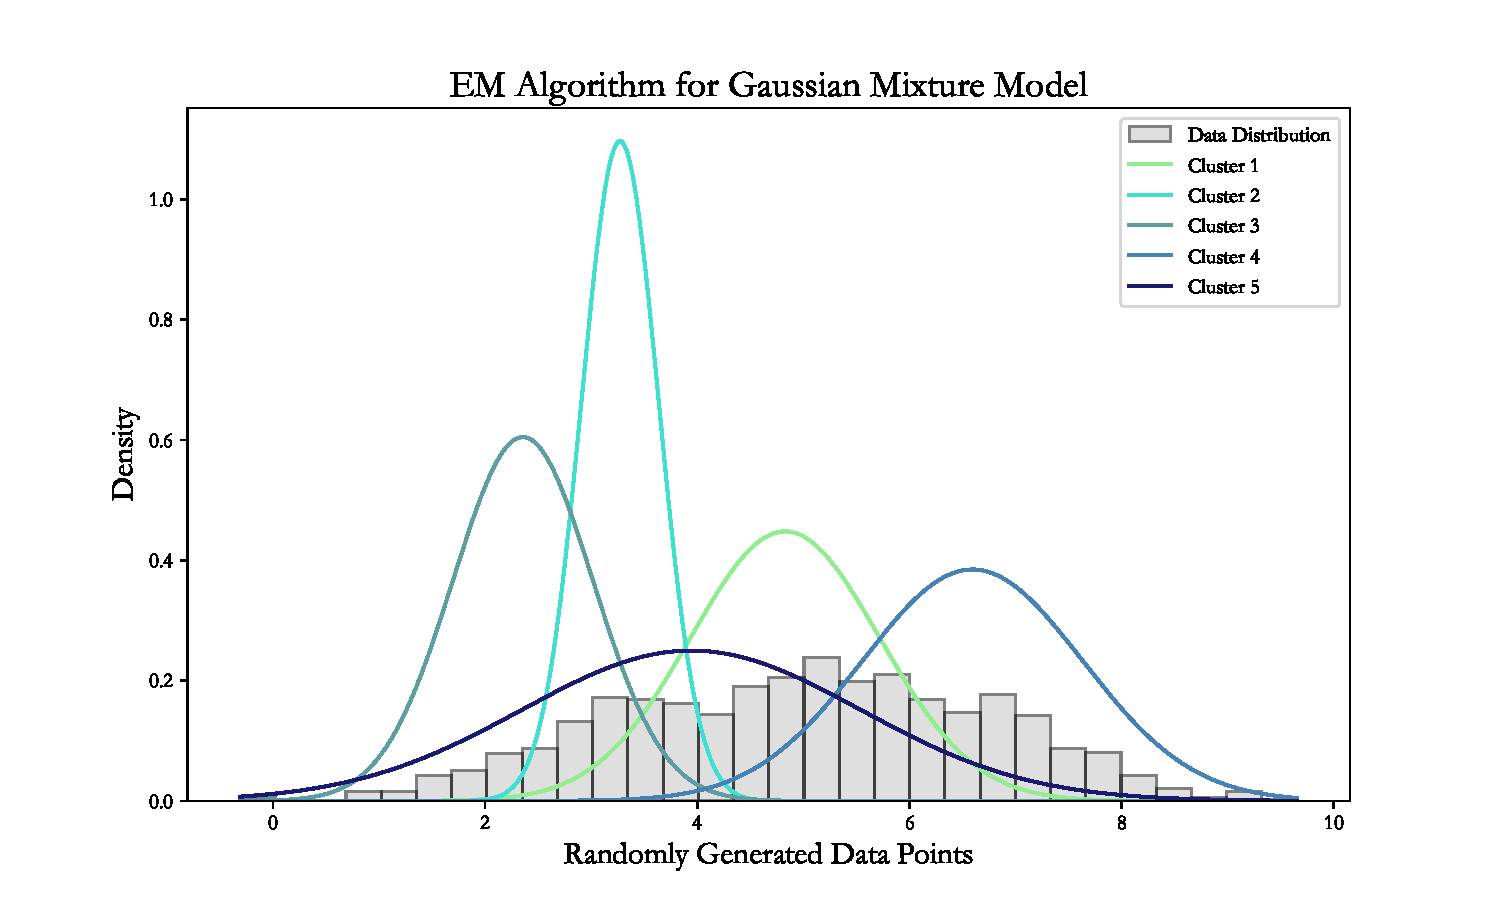
\includegraphics[width=\textwidth]{./img/EM_Gaussian_Mixture_Model.pdf}
    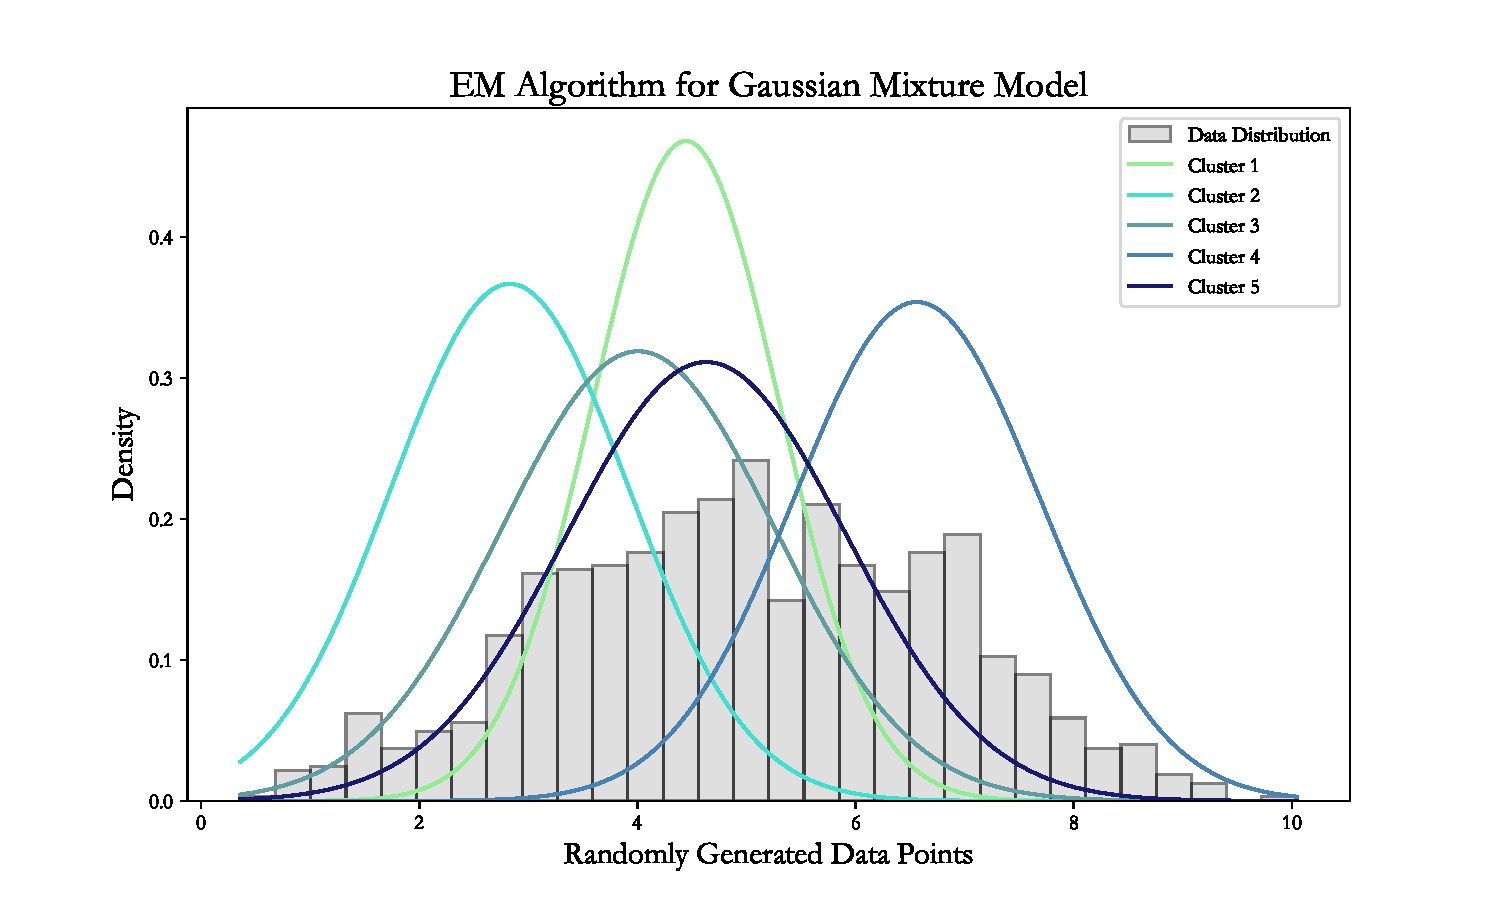
\includegraphics[width=\textwidth]{./img/em2.pdf}
    \caption{EM算法下高斯混合模型的数据分布与簇分布}
    \label{fig:EM_Gaussian_Mixture_Model}
\end{figure}

\section{验证Bartlett关于多元方差分析的抽样分布定理}
对于
\[
\begin{gathered}
    \text{总体1:}X_{11},X_{12},\hdots,X_{1n_1}\\
    \text{总体2:}X_{21},X_{22},\hdots,X_{2n_2}\\
    \vdots\\
    \text{总体k:}X_{g1},X_{g2},\hdots,X_{gn_k}\\
\end{gathered}
\]

假设每个随机变量的维数为\(p\), 当原假设\(H_0: \mu_1=\mu_2=\hdots=\mu_k\)为真时,且\(\sum_{i=1}^{g} n_{g}=n\) 充分大时,验证\(-\left(n-1-\frac{p+q}{2}\right) \ln \Lambda^\ast > \chi^2_{p(g-1)}(\alpha)\)

\subsection{计算公式}

% 1.数据产生,每人做4组
% \[g\in(3,4,\hdots,8),p\in(3,4,\hdots,30)\]
% 例如,\(g=3,p=3\)
% \[\begin{gathered}
%     \text{总体1:}[Norm,t,F]^\top\\
%     \text{总体2:}[\chi^2,\mu,Norm]^\top\\
%     \text{总体3:}[\hdots,\hdots,\hdots]^\top
% \end{gathered}\]
% 2.计算\(\lambda\),编写函数\(-(n-1-\frac{p+q}{2})\ln \Lambda\)
% 3.重复1,2步骤1000次,生成不同数据,计算\(\lambda\),拟合密度函数。\(\chi^2_{p(g-1)}(\alpha)\)
% 首先画出间隔不大的直方图,同时画出\(\chi^2_{p(g-1)}\)的概率密度曲线,观察两者是否吻合。
% 其次,画出q-q图,观察两者是否吻合。


% 协方差矩阵部分移除的显著性检验:
% 如果将\(g\)视为变量数量,\(p\)视为剩余协变量的数量,那么\(-B \ln |S-S_1|\)可被视为检验统计量,其中\(B=n-\frac{1}{2}(p+q+1)\),\(S\)是总平方和矩阵,而\(S_1\)是由其他\(q\)变量通过线性回归移除的矩阵。如果将\(q\)解释为组数减一,即\(q=g-1\),则可以推断出\(-B \ln |S-S_1|\)近似于自由度为\(pq\)的\(\chi^2\)分布。


% 为了证明命题
% \[
% -\left(n-1-\frac{p+q}{2}\right) \ln \Lambda^\ast > \chi^2_{p(g-1)}(\alpha)
% \]
% 在原假设 \(H_0: \mu_1=\mu_2=\hdots=\mu_k\) 为真时,且 \(\sum_{i=1}^{g} n_{g}=n\) 充分大的情况下,我们需回顾似然比 \(\Lambda\) 与 \(\chi^2\) 分布之间的关系,以及似然比统计量的近似性质。
\subsubsection{似然比与\(\chi^2\)分布的极限近似性}
参考Bartlett在1937年的证明。
\begin{framed}
为了在当前问题中更精确地获得\(\chi^{2}\)近似值,首先考虑\(\mu\)从方程\(C+n\log s-n\log\sigma-\frac{n}{2}\left( \frac{s^2}{\sigma^2} - 1\right)\)(即,\(k = 2\),\(n_1= n\),\(n_2=\infty\))。从已知形式的\(C+n\log s-n\log\sigma-\frac{n}{2}\left( \frac{s^2}{\sigma^2} - 1\right)\)方程关于\(s^2\)的分布,我们可以通过积分直接得到\(-2 \log \mu\)的特征函数;期望值由下式给出:
\[
M=E(\mu)^{-2t}=\frac{\Gamma[\frac{n}{2}(1-2t)](\frac{n}{2})^{nt_e-nt}}{(1-2t)^{\frac{n}{2}}\Gamma(\frac{n}{2})}
\]

设\(K=\log M\),那么近似地有:
\[
K=\sum_{k=1}^{\infty} \frac{2^{k-1} t^{k}}{k!} \left( 1+\frac{1}{3n} \right)^k
\]

如果我们将确切的函数记作\(K(n)\),那么对于一般方程\(-2\log\mu=n\log s^2-\sum n_r \log s_r^2\),由于统计量\(s_{r}^2 \mid s^{2}\)等价于与\(s^2\)独立的角度变量,
\[
K=\sum K(n_r)-K(n)
\]
或者,忽略\(O\left( {\frac{1}{n_{r}^{2}}} \right)\)项的影响,我们可以写成:
\[
-\frac{2\log\mu}{C}=\chi_{k-1}^{2},\quad C=1+\frac{1}{3(k-1)}\left(\sum\frac{1}{n_{r}}-\frac{1}{n}\right)
\]
\end{framed}

首先,根据似然比与 \(\chi^2\) 分布之间的极限关系,当样本量 \(n \rightarrow \infty\) 时,似然比统计量的分布趋向于 \(\chi^2_{pq}\) 分布。
\[
2 \log \Lambda^{\frac{1}{2}n} = - n \log \Lambda
\]

\subsubsection{特征函数的推导}

进一步考察近似值,我们得到 \(- n\log A\) 的特征函数 \(M\),\(K\)的近似表达式通过对\(M\)的对数进行级数展开得到。
\[
\begin{gathered}
M=\prod_{i=0}^{p-1} \frac{\Gamma(\frac{1}{2}(n-i)) \Gamma(\frac{1}{2}(n-q-i)-nt) }{\Gamma(\frac{1}{2}(n-q-i)) \Gamma(\frac{1}{2}(n-i)-nt)}\\
K=\log M=\sum_{i=0}^{p-1} K(i)
\end{gathered}
\]

\subsubsection{近似公式的提出}

由 \(\Gamma\)-函数的斯特林(Stirling)公式展开,可得对于特殊情况 \(p = 1\), \(q = 2\)(或等价地,\(p = 2\), \(q = 1\)),\(\Lambda\) 的分布为
\[
p(\Lambda) \propto \Lambda^{\frac{1}{2}(n-2)}d \log \Lambda
\]

因此 \(\chi^2=-(n-2) \log \Lambda\) 确切成立。

从而一般情况下提出了近似公式
\[
\chi_1^2=-\left(n-\frac{1}{2}(p+q+1)\right) \log \Lambda
\]

\subsubsection{多元方差分析的应用}

现在,考虑命题中的 \(\Lambda^\ast\),它指的是在多组均值相等的原假设下计算的似然比统计量。根据上述分析,当 \(n\) 充分大时,\(\Lambda^\ast\) 的对数值乘以一个适当的系数应当近似服从自由度为 \(p(g-1)\) 的 \(\chi^2\) 分布。这意味着
\[
-\left(n-1-\frac{p+q}{2}\right) \ln \Lambda^\ast \sim \chi^2_{p(g-1)}(\alpha)
\]

综上所述,若 \(-\left(n-1-\frac{p+q}{2}\right) \ln \Lambda^\ast\) 大于 \(\chi^2_{p(g-1)}(\alpha)\),则说明在 \(H_0\) 成立的情况下,观察到的 \(\Lambda^\ast\) 值导致的似然比统计量落在 \(\chi^2\) 分布的尾部区域,这表明我们有足够的理由怀疑原假设的真实性。因此,这个命题实质上是在描述如何通过似然比检验来评估多组均值是否相等的假设。

\newpage

\subsection{编程实现}

\begin{lstlisting}
from scipy.stats import chi2
import numpy as np
import matplotlib.pyplot as plt

# 绘制 Q-Q 图
def plot_qq(data, p, g, df):
    plt.rcParams['font.family'] = 'Garamond'
    # Step1: 排序,计算概率
    nums = len(data)
    probability = (np.arange(1, nums + 1) - 0.5) / nums
    sorted_data = sorted(data)

    # Step2: 计算分位数对应的值
    normal_data = chi2.ppf(probability, df)

    # Step3: 画图
    plt.scatter(sorted_data, normal_data, s=3, color='midnightblue')  # 调整点的大小为10,颜色为darkblue
    plt.title(f'Q-Q Plot For X^2 Sample p={p}, g={g}', fontsize=18)

    # 添加拟合直线
    z = np.polyfit(sorted_data, normal_data, 1)
    pp = np.poly1d(z)
    plt.plot(sorted_data, pp(sorted_data), color='crimson', linewidth=0.7)  # 拟合直线颜色为crimson

    plt.savefig(f"qq_plot_p={p}_g={g}.pdf", format='pdf')
    plt.clf()

# 绘制直方图和卡方分布的概率密度函数
def plot_hist_chi(plot_data, p, g):
    # 画直方图
    plt.rcParams['font.family'] = 'Garamond'
    plt.hist(plot_data, bins=30, density=True, alpha=0.6, color='lightgray', edgecolor='black', label='Data Distribution')

    # 生成卡方分布的概率密度函数
    x = np.linspace(min(plot_data), max(plot_data), 10000)
    df = p * (g - 1)
    pdf = chi2.pdf(x, df=df)

    # 叠加卡方分布的概率密度函数
    plt.plot(x, pdf, color='darkblue', label='Chi-Square PDF')

    # 设置坐标轴标签和标题
    plt.xlabel('Value', fontsize=15)
    plt.ylabel('Density', fontsize=15)
    plt.title(f'Histogram and Chi-Square PDF p={p}, g={g}', fontsize=18)
    plt.legend()

    # 保存图像
    plt.savefig(f"hist_plot_p={p}_g={g}.pdf", format="pdf")

    # 清除缓存,以便于绘制新的图像
    plt.clf()

# 统计分布采样选择函数
def sample_dist(size, dist=None):
    if dist == 'N':  # 正态分布
        return np.random.normal(loc=0, scale=0.1, size=size)
    elif dist == 'U':  # 均匀分布
        return np.random.uniform(low=-1, high=1, size=size)
    elif dist == 'P':  # 泊松分布
        return np.random.poisson(lam=5, size=size)
    elif dist == 'E':  # 指数分布
        return np.random.exponential(scale=5, size=size)
    elif dist == 'T':  # 标准t分布
        return np.random.standard_t(df=3, size=size)
    elif dist == 'X2':  # 卡方分布
        return np.random.chisquare(df=7, size=size)
    else:
        raise ValueError('Unknown distribution')


# 计算 Wilks' Lambda
def calc_wilks_lambda(data, p, g, N):
    group_means = np.mean(data, axis=2)  # group_means: [g, p]
    overall_means = np.mean(data, axis=(0, 2))  # overall_means: [p]

    # 计算组均值与总体均值之间的差异
    group_mean_diff = (group_means - overall_means[None, :])[:, :, None]  # group_mean_diff: [g, p, 1]
    group_mean_diff_transpose = (group_means - overall_means[None, :])[:, None, :]  # group_mean_diff_transpose: [g, 1, p]

    # 计算组间散布矩阵 B
    B = (group_mean_diff @ group_mean_diff_transpose).sum(axis=0) * N

    # 计算观测值与对应组均值之间的差异
    within_group_diff = (data - group_means[:, :, None]).transpose(0, 2, 1)[:, :, :, None]  # within_group_diff: [g, N, p, 1]
    within_group_diff_transpose = (data - group_means[:, :, None]).transpose(0, 2, 1)[:, :, None, :]  # within_group_diff_transpose: [g, N, 1, p]

    # 组内散布矩阵 W
    W = (within_group_diff @ within_group_diff_transpose).sum(axis=(0, 1))

    # 计算 Wilks' Lambda
    lambda_val = np.linalg.det(W) / np.linalg.det(B + W)

    return -(g * N - 1 - (p + g) / 2) * np.log(lambda_val)


# 迭代函数
def perform_iter(P, G, N, Step, pdf_list):
    for p in P:
        for g in G:
            plot_data = []
            for step in range(Step):
                all_data = []

                name_list = np.random.choice(pdf_list, size=p, replace=True)
                for index in range(g):
                    data_list = [sample_dist(N, name_list[idx])[None, :] for idx in range(p)]
                    data = np.concatenate(data_list)
                    all_data.append(data[None, :])

                data = np.concatenate(all_data)  # data: [g, p, N]

                result = calc_wilks_lambda(data, p, g, N)
                plot_data.append(result)

            plot_hist_chi(plot_data, p, g)
            plot_qq(plot_data, p, g, df=p * (g - 1))

if __name__ == '__main__':
    G = [3, 5, 7]
    P = [3, 10, 20, 30]
    N = 1000
    Step = 2000
    pdf_list = ['N', 'U', 'P', 'E', 'T', 'X2']  # 可选的分布

    # 调用函数进行迭代
    perform_iter(P, G, N, Step, pdf_list)
\end{lstlisting}

\newpage
\subsection{测试结果}

更换不同的组数和变量数,我们可以得到不同的直方图和 Q-Q 图,以及卡方分布的概率密度函数。

下面展示了其中12组的测试结果,抽样统计量\(\Lambda^\ast\)与理论分布\(\chi^2\)分布十分吻合;Q-Q图上的点大致落在\(y=x\)直线上,说明样本数据的分位数与理论分布的分位数相符。

综上,实验结果可验证Bartlett关于多元方差分析的抽样分布定理。

\begin{figure}[H]
    \centering
    % 第一二行
    \begin{minipage}[b]{0.49\textwidth}
        \centering
        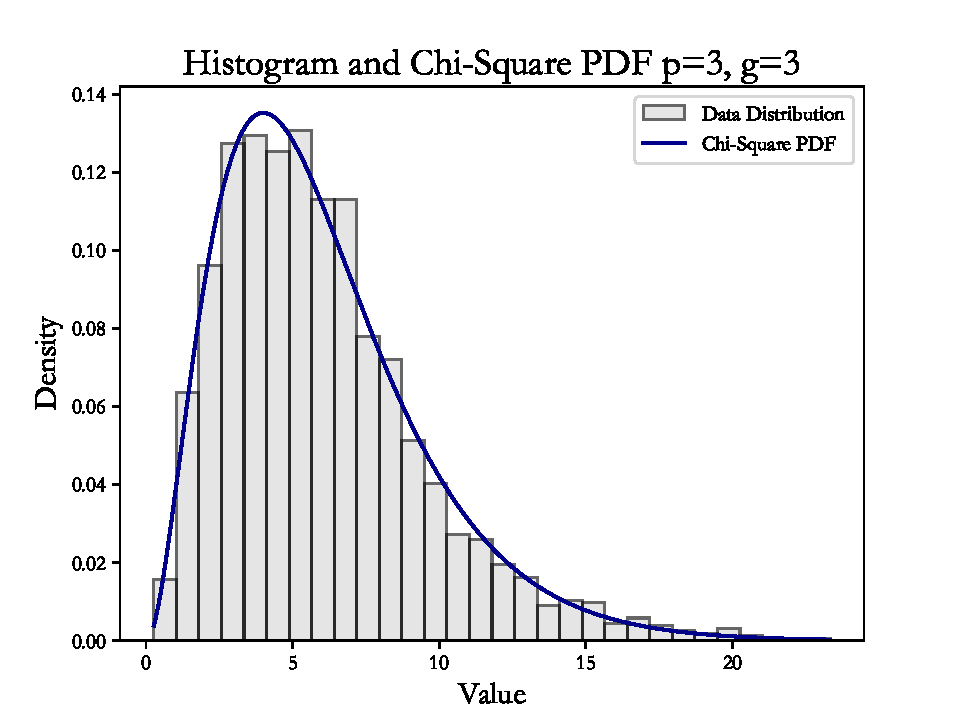
\includegraphics[width=\textwidth]{img/b/hist_plot_p=3_g=3.pdf}
    \end{minipage}
    \hfill
    \begin{minipage}[b]{0.49\textwidth}
        \centering
        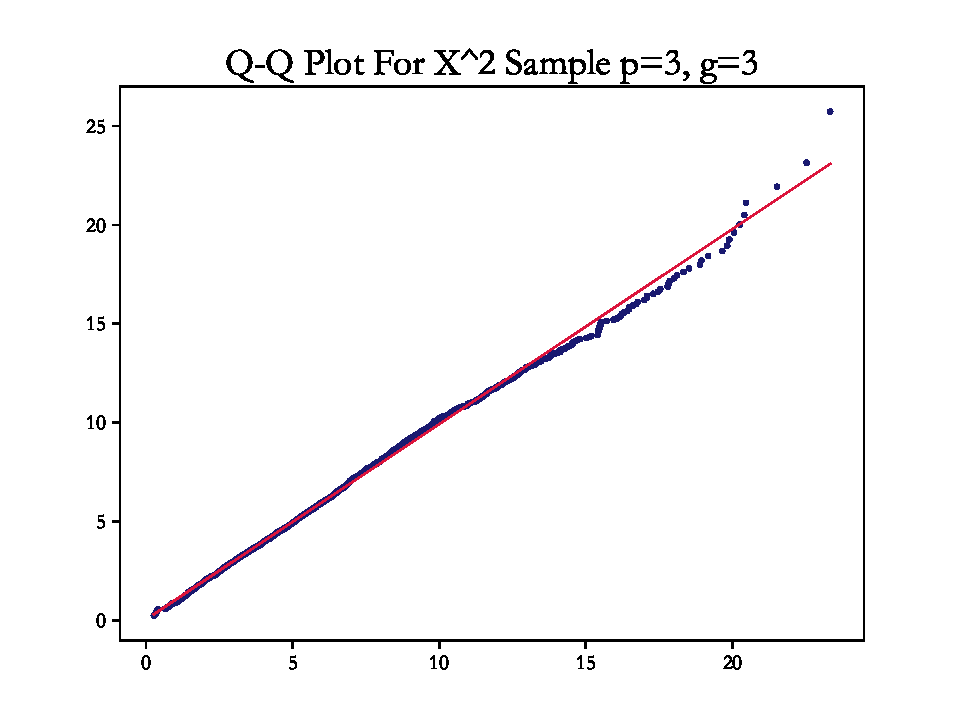
\includegraphics[width=\textwidth]{img/b/qq_plot_p=3_g=3.pdf}
    \end{minipage}
    \hfill
    \begin{minipage}[b]{0.49\textwidth}
        \centering
        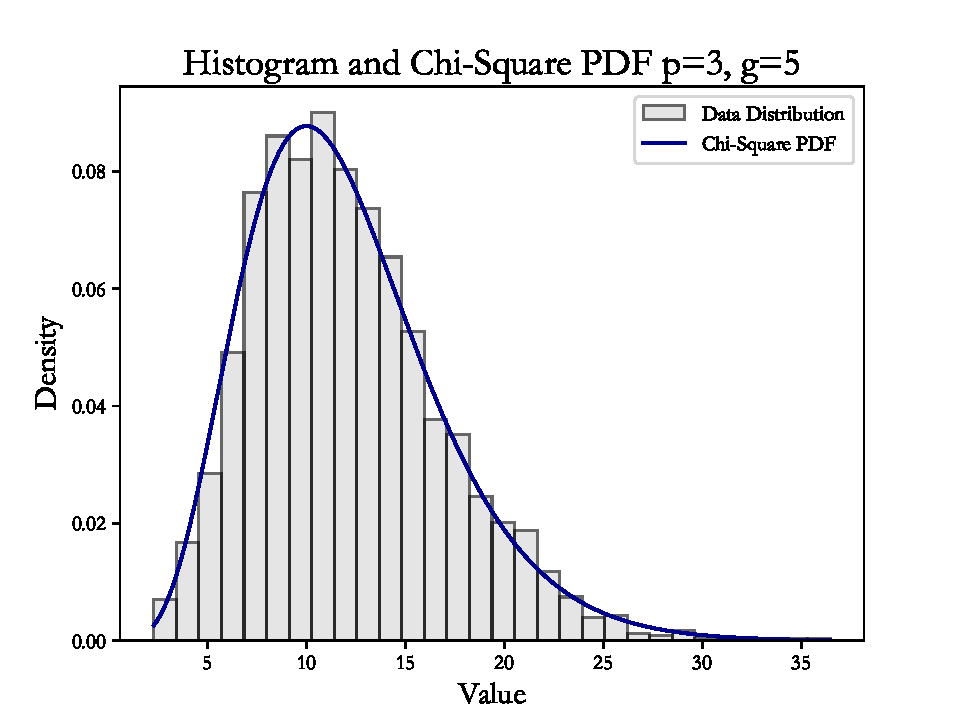
\includegraphics[width=\textwidth]{img/b/hist_plot_p=3_g=5.pdf}
    \end{minipage}
    \hfill
    \begin{minipage}[b]{0.49\textwidth}
        \centering
        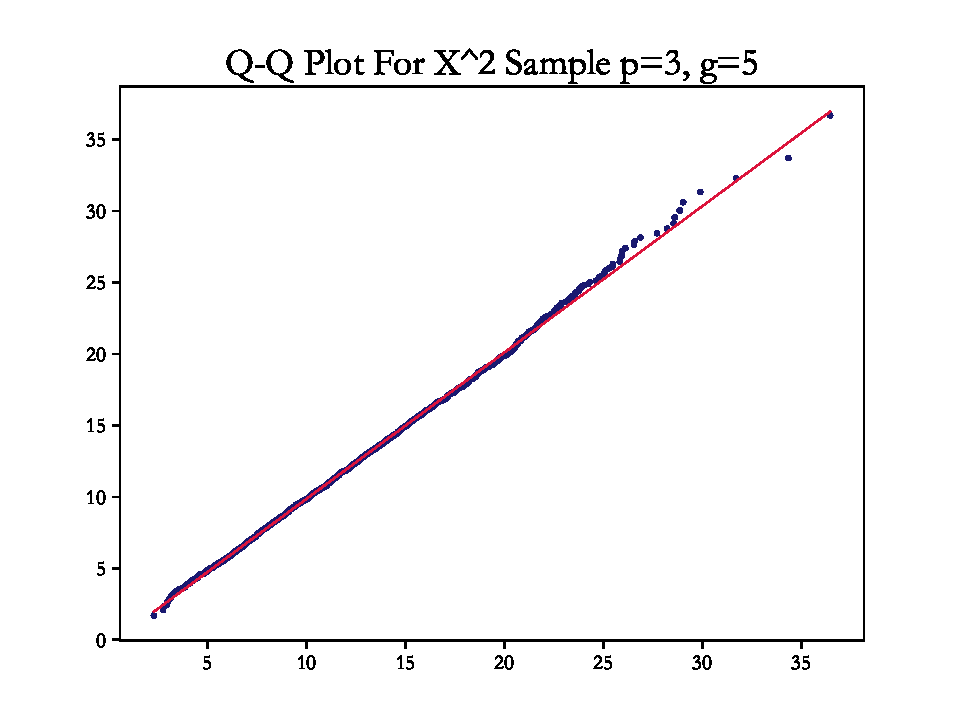
\includegraphics[width=\textwidth]{img/b/qq_plot_p=3_g=5.pdf}
    \end{minipage}
    
    % 第三四行
    \begin{minipage}[b]{0.49\textwidth}
        \centering
        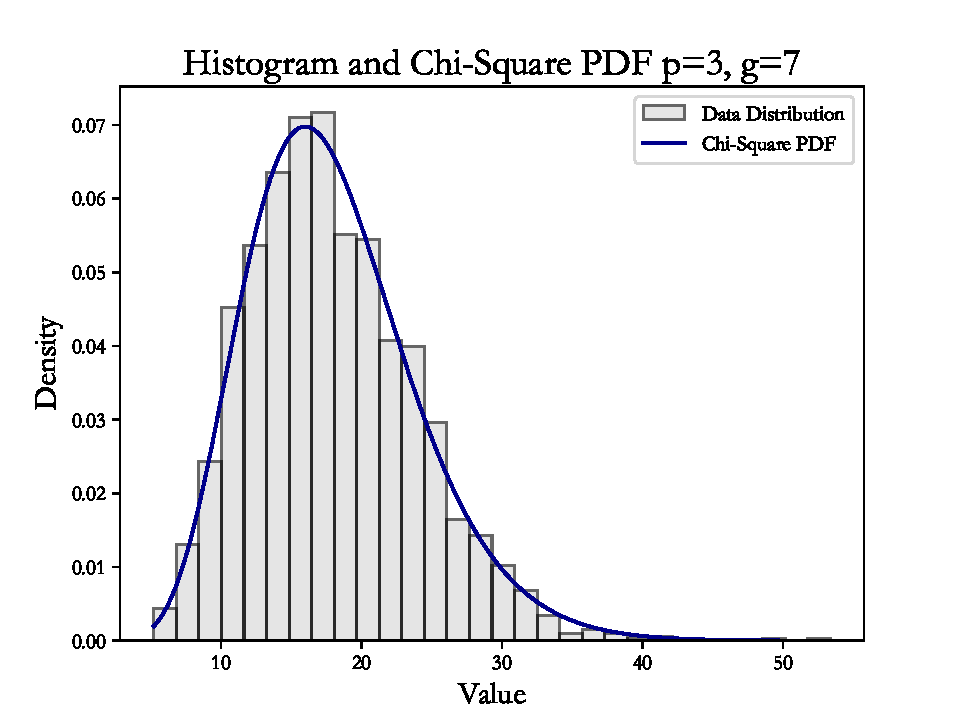
\includegraphics[width=\textwidth]{img/b/hist_plot_p=3_g=7.pdf}
    \end{minipage}
    \hfill
    \begin{minipage}[b]{0.49\textwidth}
        \centering
        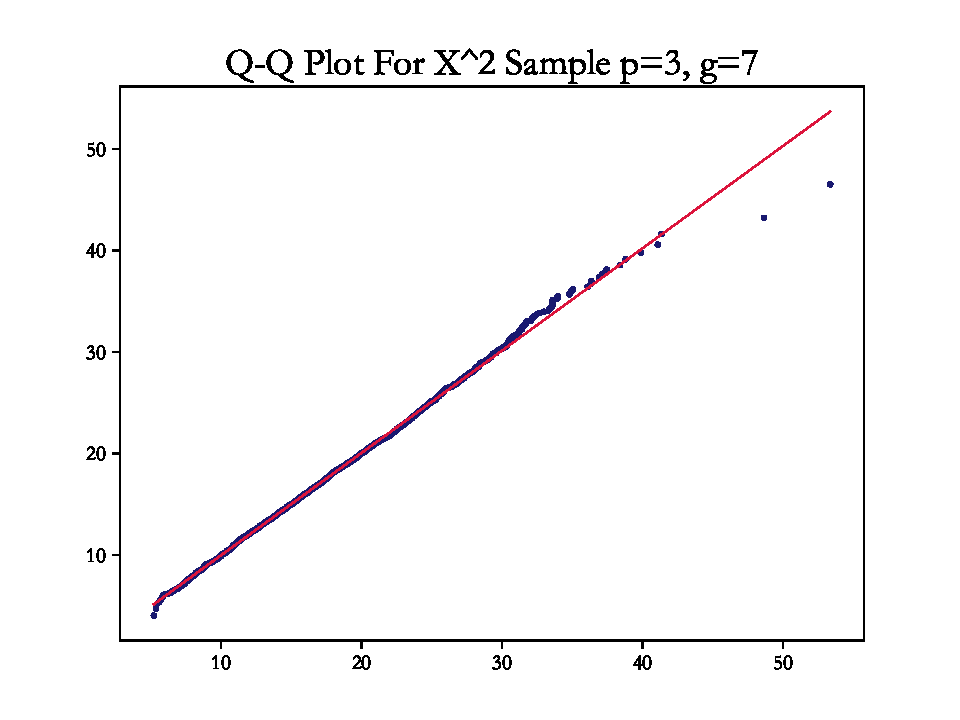
\includegraphics[width=\textwidth]{img/b/qq_plot_p=3_g=7.pdf}
    \end{minipage}
    \caption{当\(p=3\), \(g=3,5,7\)时的测试结果}
    \label{fig:collection1}
\end{figure}

\begin{figure}[H]
    \centering
    % 第一二行
    \begin{minipage}[b]{0.49\textwidth}
        \centering
        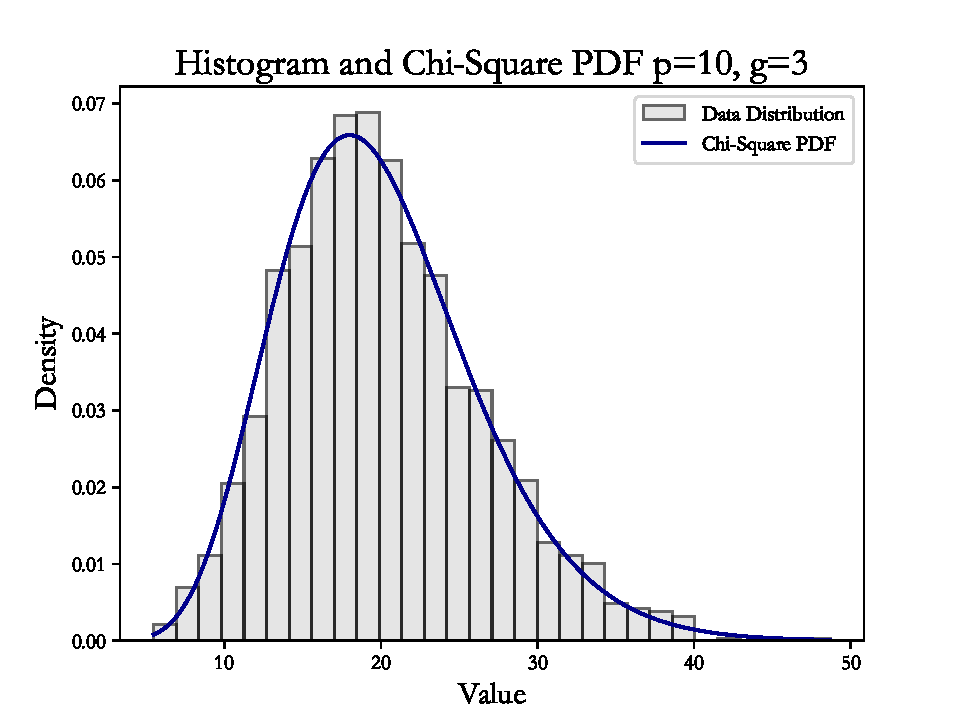
\includegraphics[width=\textwidth]{img/b/hist_plot_p=10_g=3.pdf}
    \end{minipage}
    \hfill
    \begin{minipage}[b]{0.49\textwidth}
        \centering
        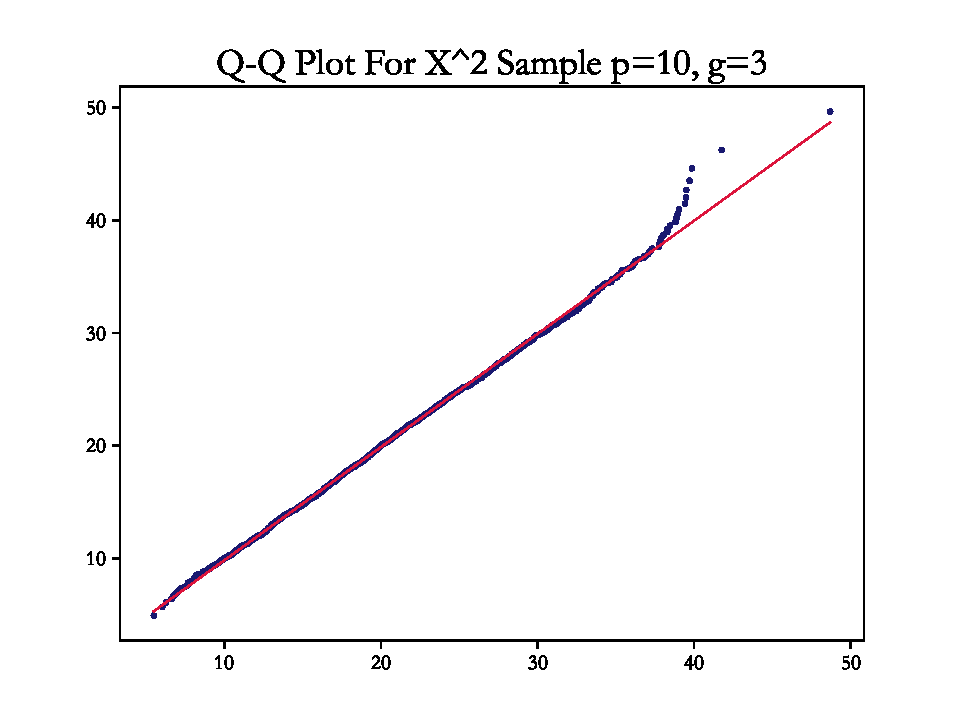
\includegraphics[width=\textwidth]{img/b/qq_plot_p=10_g=3.pdf}
    \end{minipage}
    \hfill
    \begin{minipage}[b]{0.49\textwidth}
        \centering
        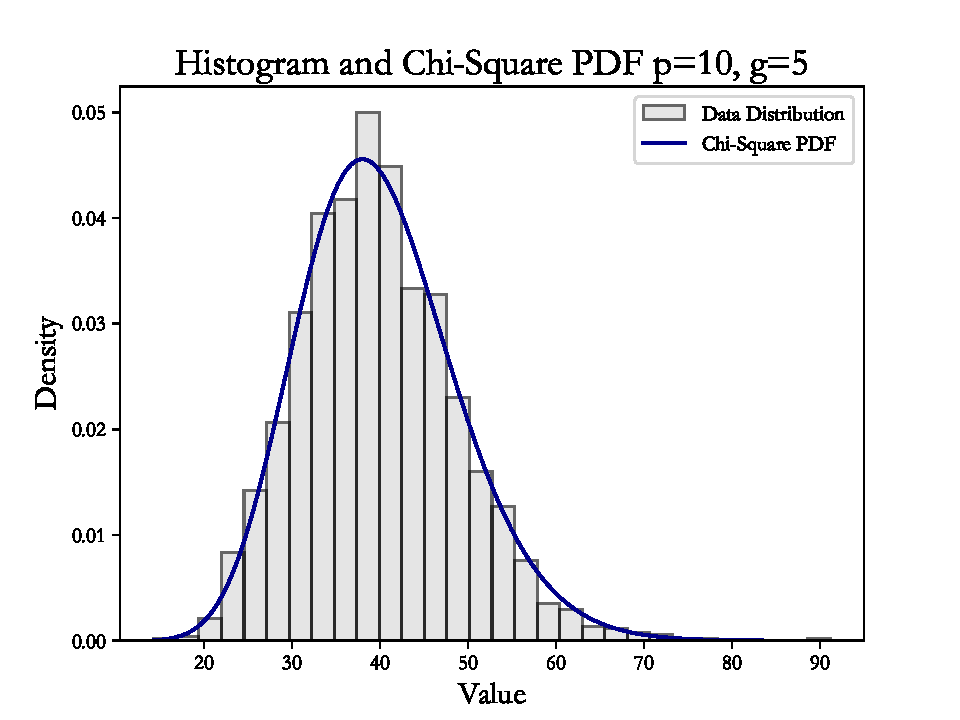
\includegraphics[width=\textwidth]{img/b/hist_plot_p=10_g=5.pdf}
    \end{minipage}
    \hfill
    \begin{minipage}[b]{0.49\textwidth}
        \centering
        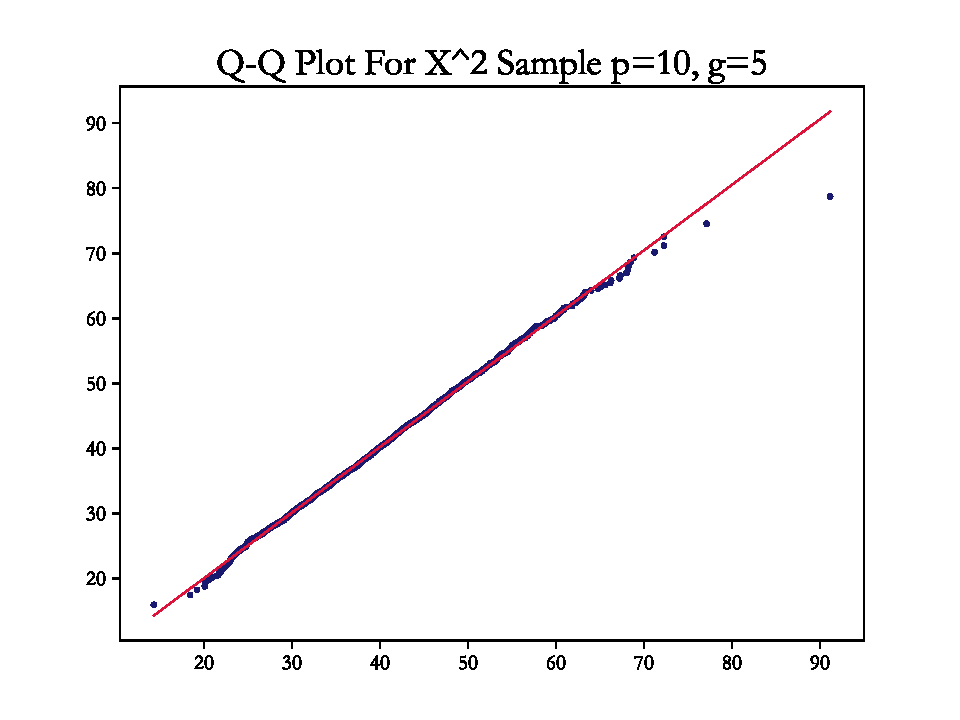
\includegraphics[width=\textwidth]{img/b/qq_plot_p=10_g=5.pdf}
    \end{minipage}
    \hfill
    \begin{minipage}[b]{0.49\textwidth}
        \centering
        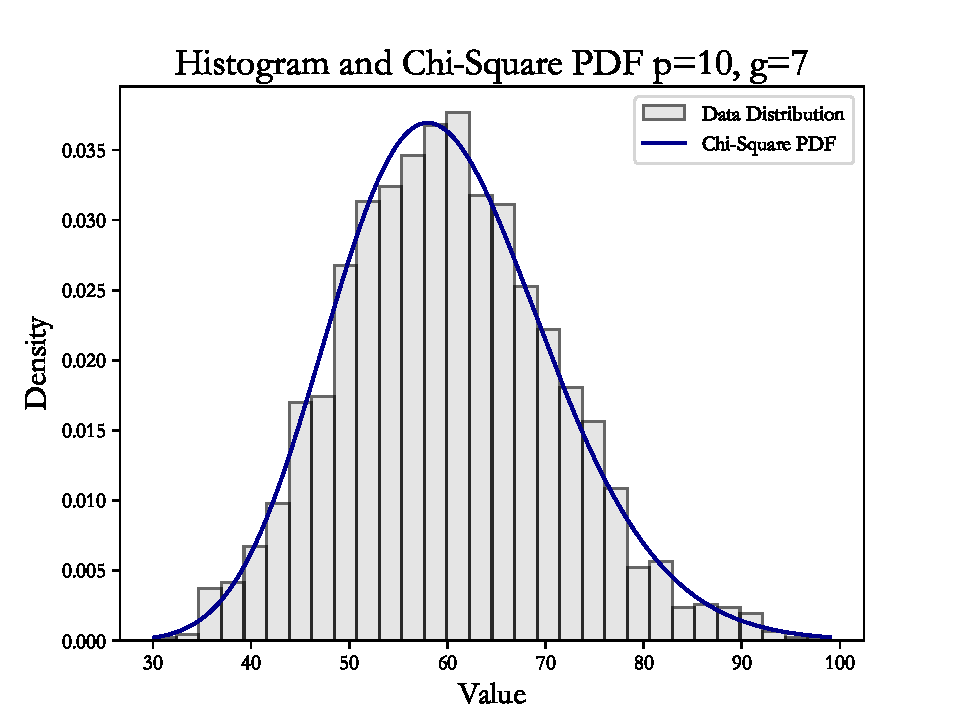
\includegraphics[width=\textwidth]{img/b/hist_plot_p=10_g=7.pdf}
    \end{minipage}
    \hfill
    \begin{minipage}[b]{0.49\textwidth}
        \centering
        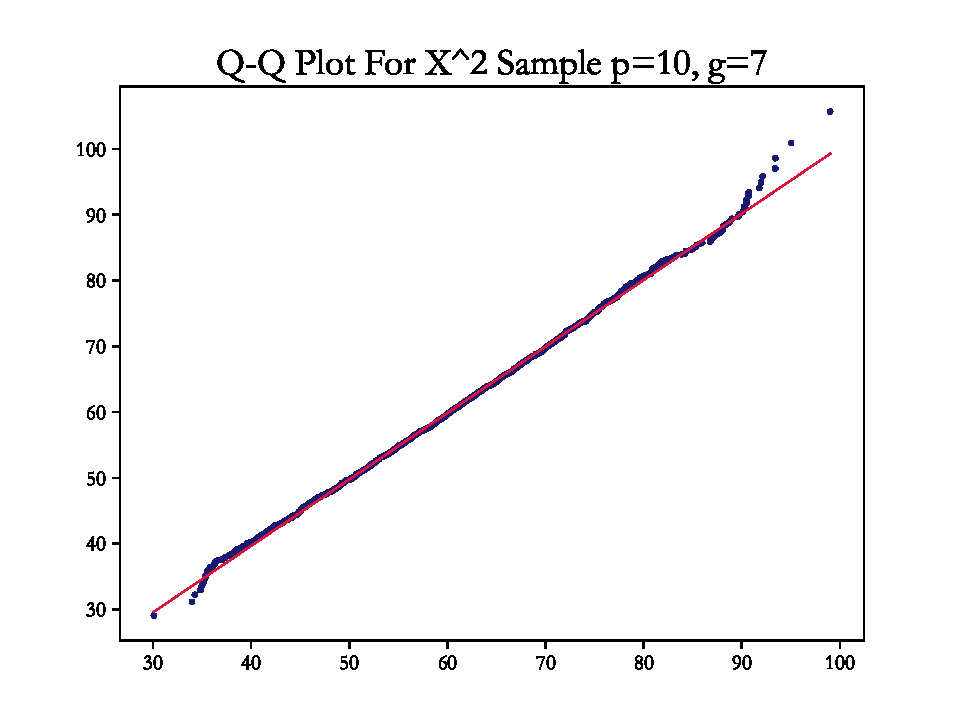
\includegraphics[width=\textwidth]{img/b/qq_plot_p=10_g=7.pdf}
    \end{minipage}

    \caption{当\(p=10\), \(g=3,5,7\)时的测试结果}
    \label{fig:collection2}
\end{figure}

\begin{figure}[H]
    \centering
    \begin{minipage}[b]{0.49\textwidth}
        \centering
        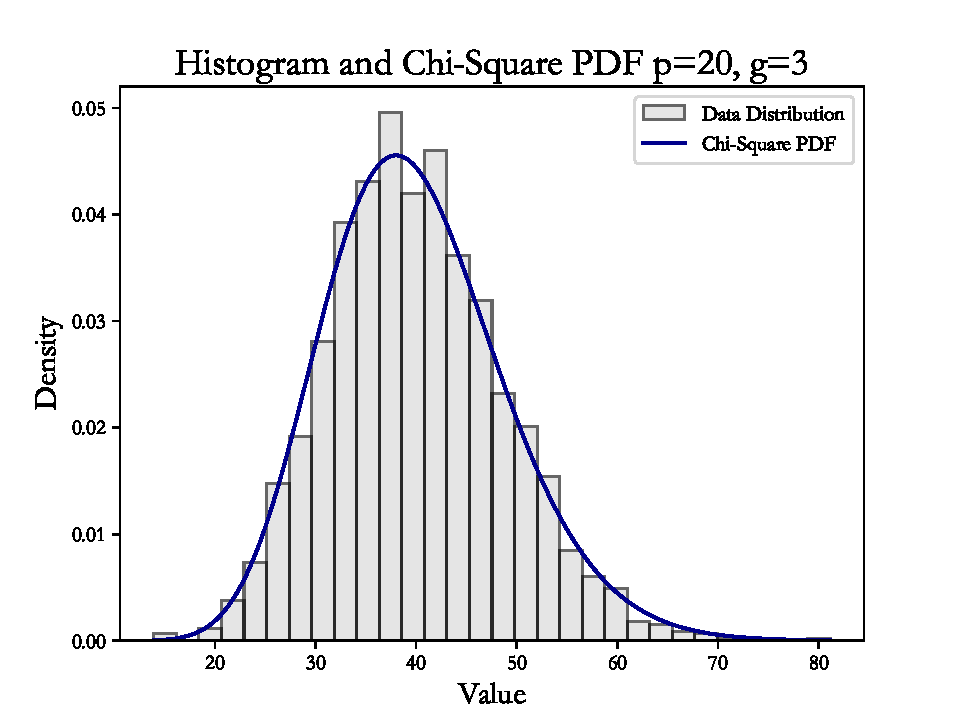
\includegraphics[width=\textwidth]{img/b/hist_plot_p=20_g=3.pdf}
    \end{minipage}
    \hfill
    \begin{minipage}[b]{0.49\textwidth}
        \centering
        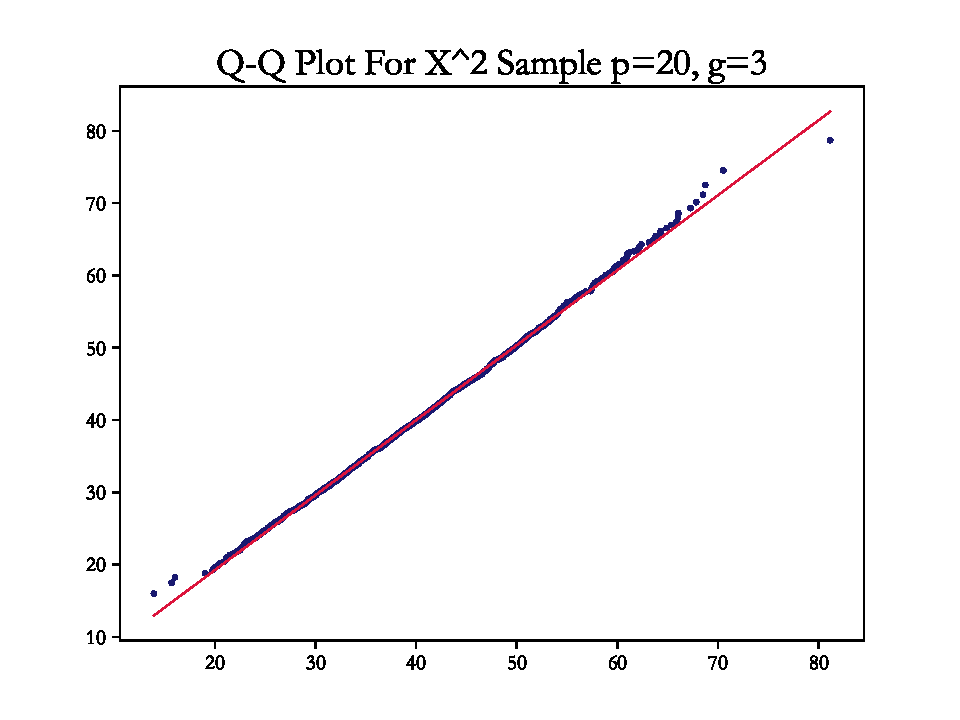
\includegraphics[width=\textwidth]{img/b/qq_plot_p=20_g=3.pdf}
    \end{minipage}
    \hfill
    \begin{minipage}[b]{0.49\textwidth}
        \centering
        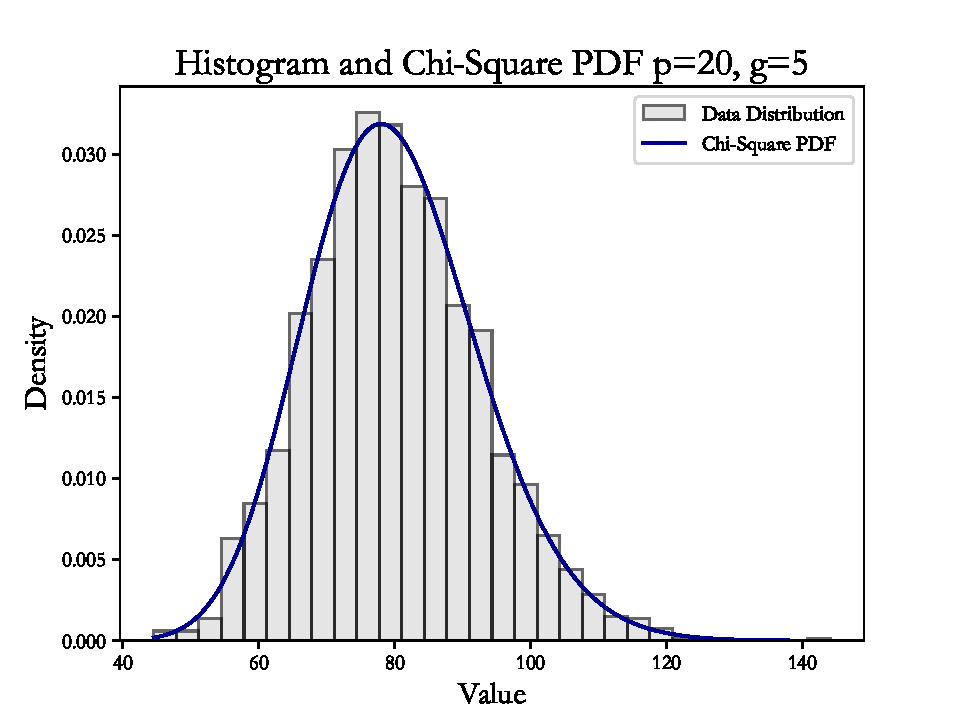
\includegraphics[width=\textwidth]{img/b/hist_plot_p=20_g=5.pdf}
    \end{minipage}
    \hfill
    \begin{minipage}[b]{0.49\textwidth}
        \centering
        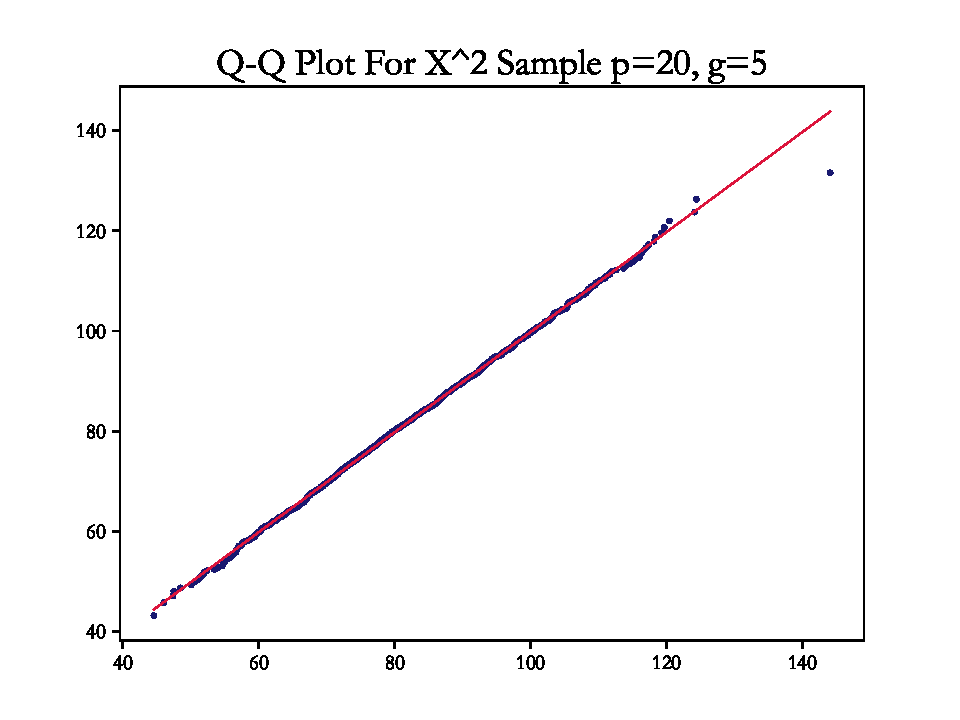
\includegraphics[width=\textwidth]{img/b/qq_plot_p=20_g=5.pdf}
    \end{minipage}
    \hfill
    \begin{minipage}[b]{0.49\textwidth}
        \centering
        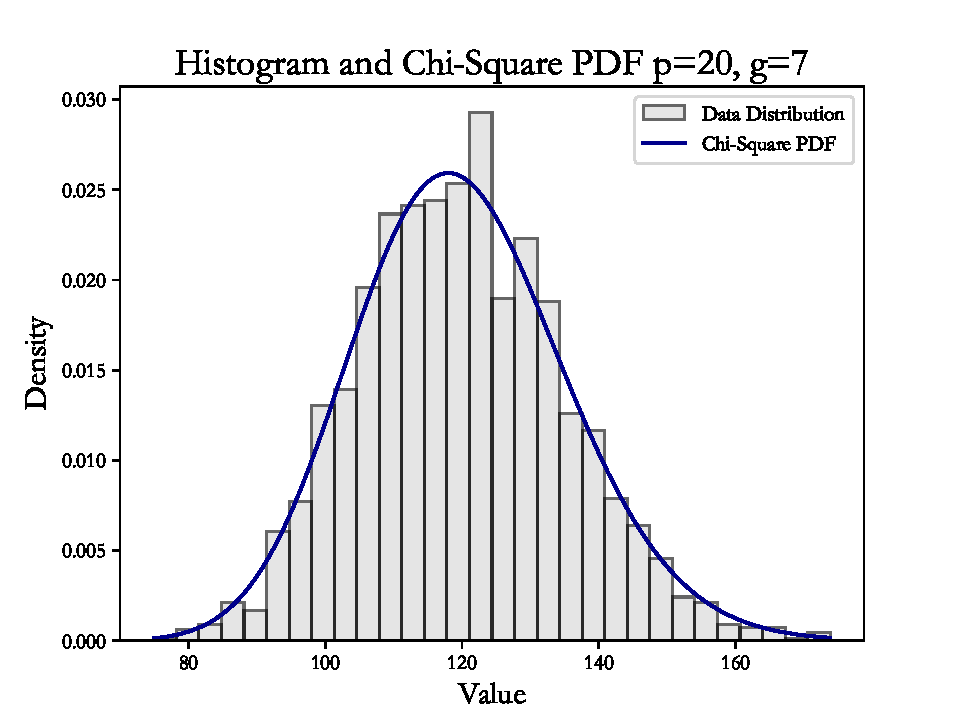
\includegraphics[width=\textwidth]{img/b/hist_plot_p=20_g=7.pdf}
    \end{minipage}
    \hfill
    \begin{minipage}[b]{0.49\textwidth}
        \centering
        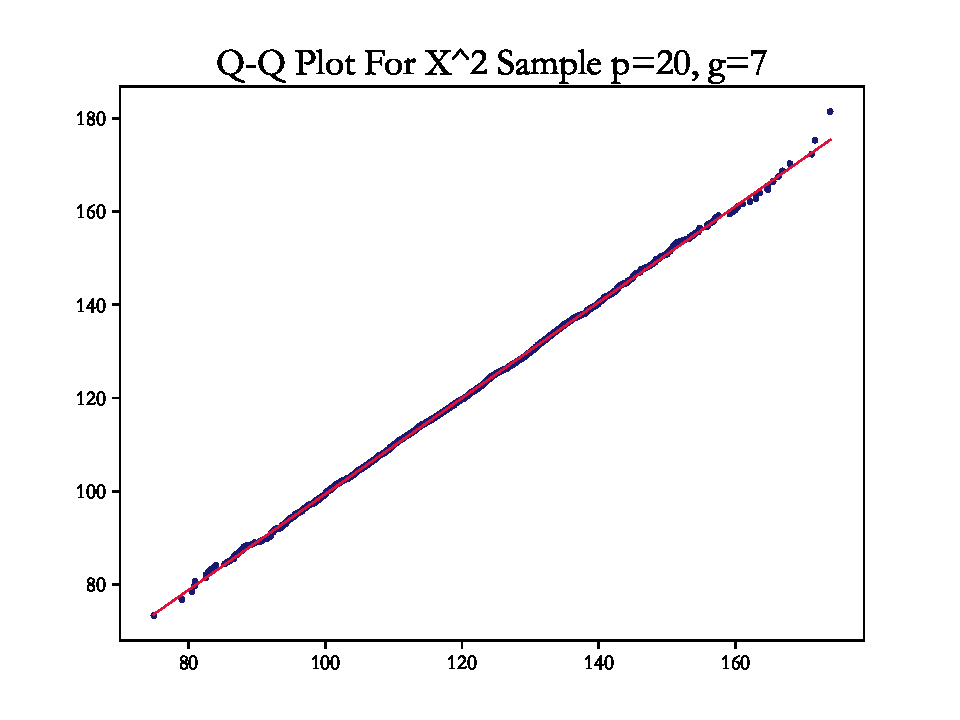
\includegraphics[width=\textwidth]{img/b/qq_plot_p=20_g=7.pdf}
    \end{minipage}
    \caption{当\(p=20\), \(g=3,5,7\)时的测试结果}
    \label{fig:collection3}
\end{figure}

\begin{figure}[H]
    \centering
    \begin{minipage}[b]{0.49\textwidth}
        \centering
        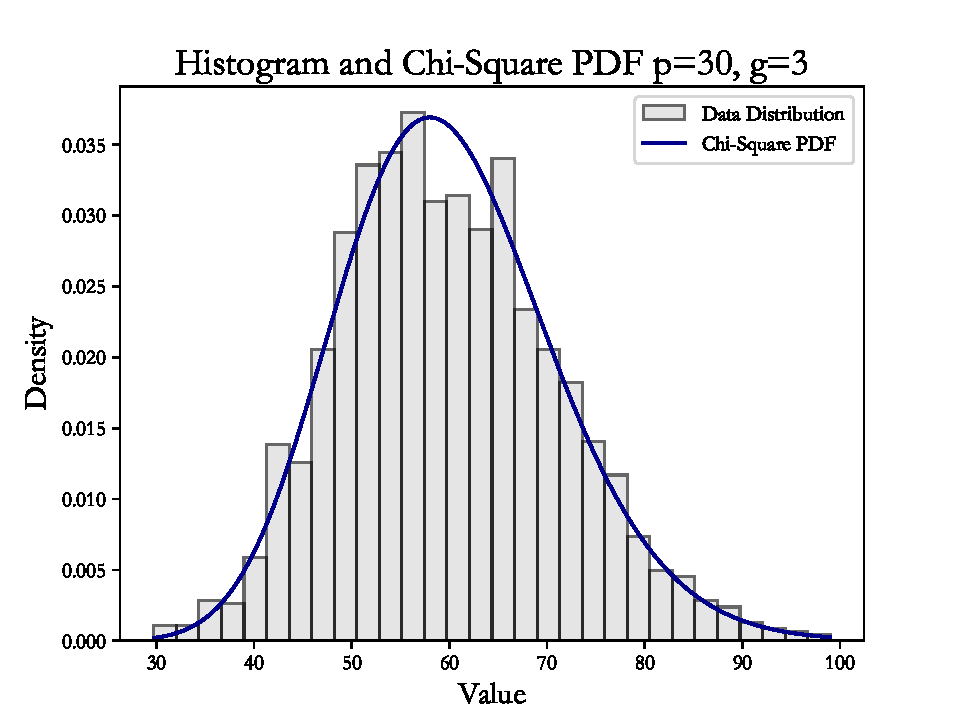
\includegraphics[width=\textwidth]{img/b/hist_plot_p=30_g=3.pdf}
    \end{minipage}
    \hfill
    \begin{minipage}[b]{0.49\textwidth}
        \centering
        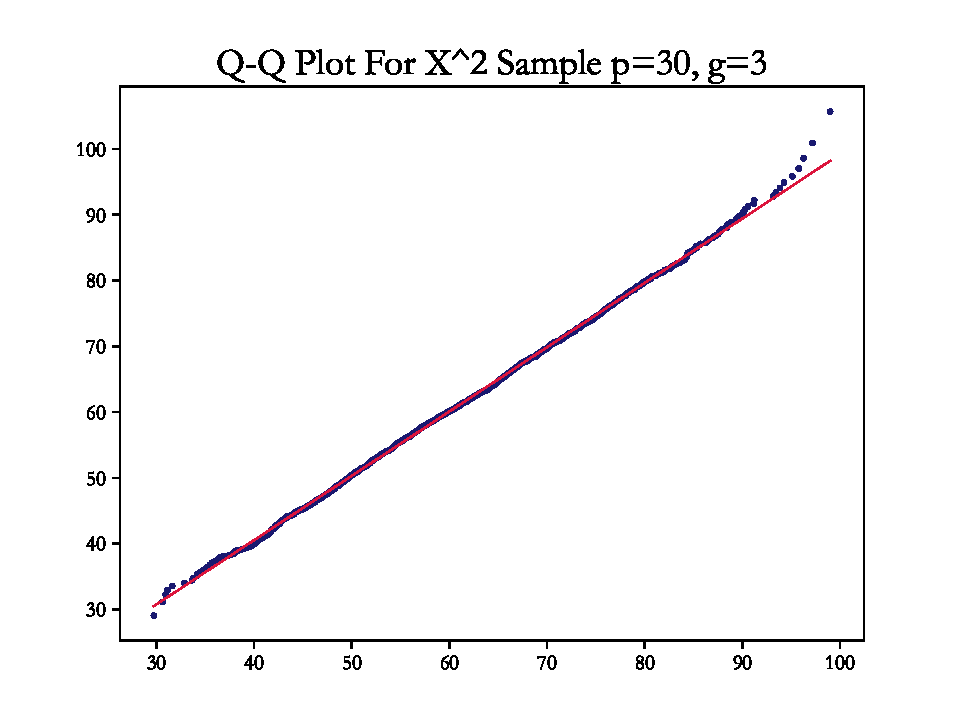
\includegraphics[width=\textwidth]{img/b/qq_plot_p=30_g=3.pdf}
    \end{minipage}
    
    % 第三四行
    \begin{minipage}[b]{0.49\textwidth}
        \centering
        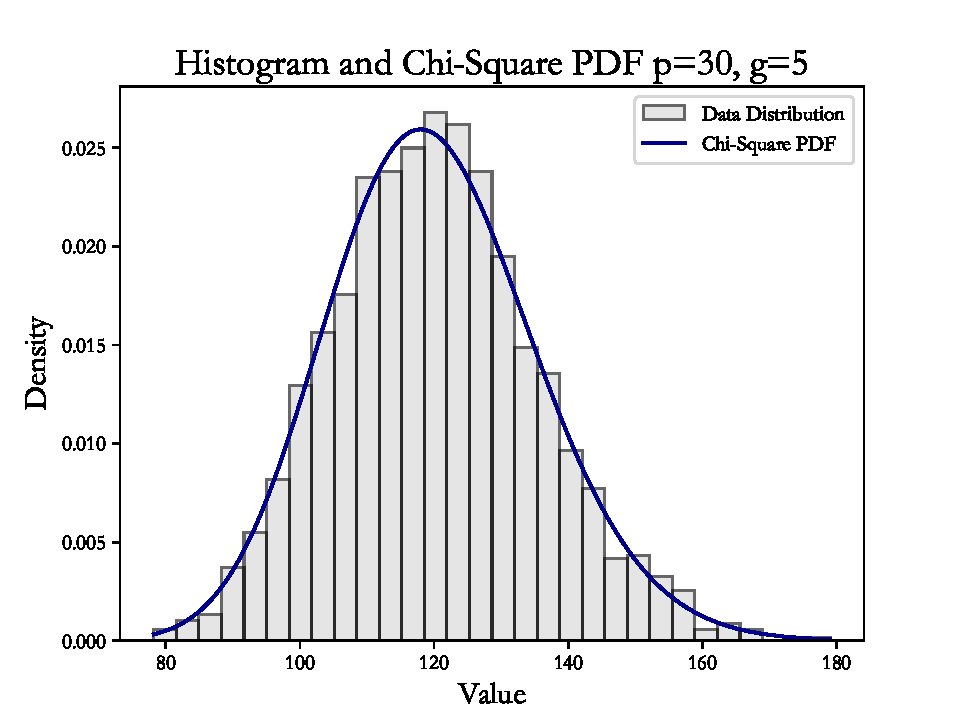
\includegraphics[width=\textwidth]{img/b/hist_plot_p=30_g=5.pdf}
    \end{minipage}
    \hfill
    \begin{minipage}[b]{0.49\textwidth}
        \centering
        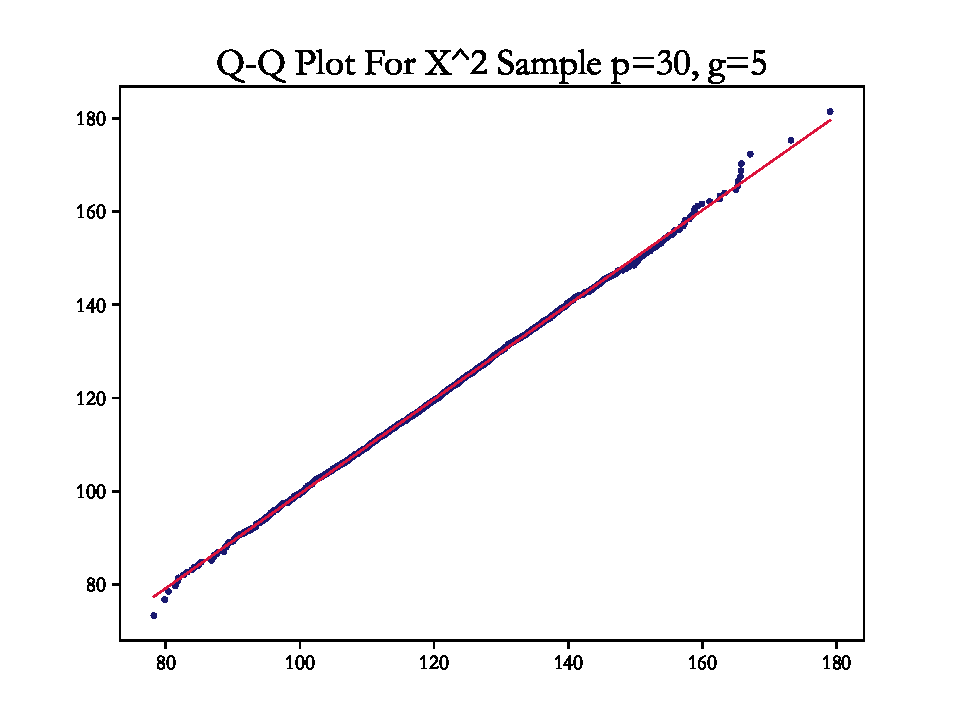
\includegraphics[width=\textwidth]{img/b/qq_plot_p=30_g=5.pdf}
    \end{minipage}
    \hfill
    \begin{minipage}[b]{0.49\textwidth}
        \centering
        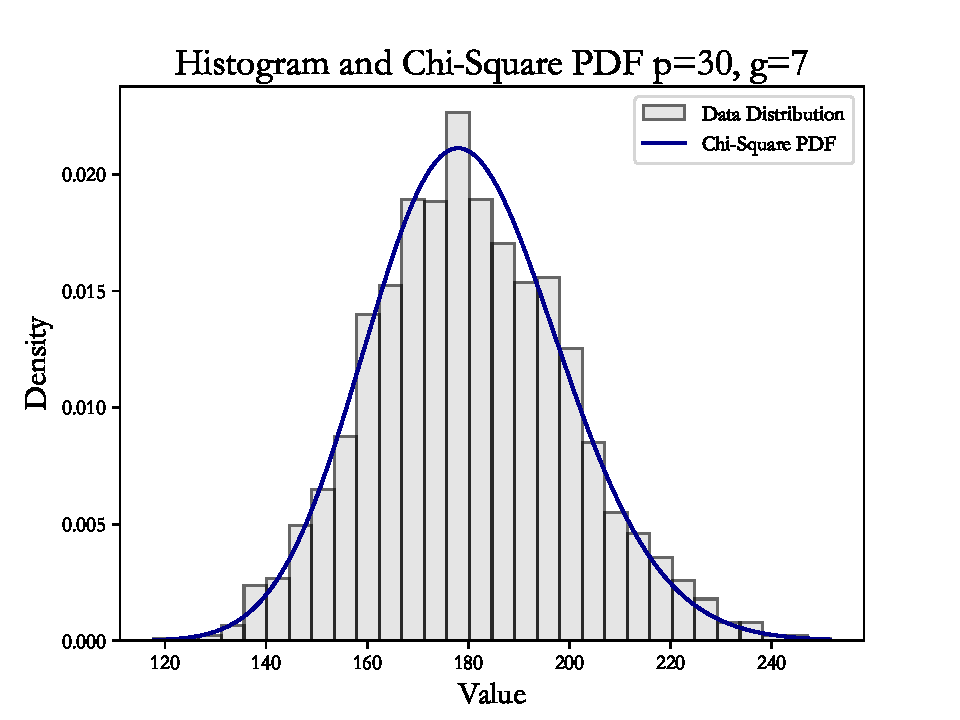
\includegraphics[width=\textwidth]{img/b/hist_plot_p=30_g=7.pdf}
    \end{minipage}
    \hfill
    \begin{minipage}[b]{0.49\textwidth}
        \centering
        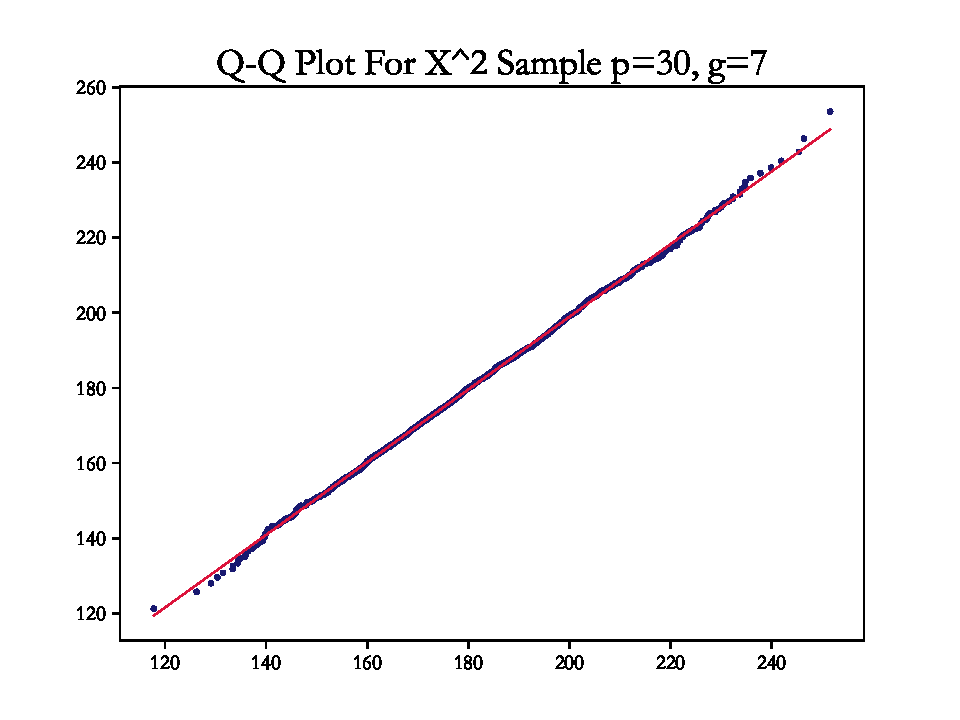
\includegraphics[width=\textwidth]{img/b/qq_plot_p=30_g=7.pdf}
    \end{minipage}
    \caption{当\(p=30\), \(g=3,5,7\)时的测试结果}
    \label{fig:collection4}
\end{figure}



\end{document}